\subsection{Respuesta en frecuencia del circuito}

\subsubsection{An\'alisis te\'orico} %%%%%%%

\subsubsection*{Configuraci\'on inversora}
Se calcula de forma te\'orica la ganancia del circuito \ref{c1}, considerando al amplificador operacional como ideal, es decir, con impedancia de entrada infinita, impedancia de salida nula y masa virtual en la terminal de entrada $V^{-}$. Se parte de las siguientes ecuaciones:
\begin{equation}
	\begin{cases}
		V_{out} = A_{vol}\cdot(V^+ - V^-) = -A_{vol}\\
		V_{in} - R_1 \cdot I_1 = V^- \\
		V_{out} - R_2 \cdot I_2 = V^- 
	\end{cases}
	\label{ecsbase}
\end{equation}

Operando matem\'aticamente se obtiene la siguiente expresi\'on:

\begin{equation}
	\frac{V{out}}{V_{in}} = - \frac{R_2/R_1}{1 + \frac{R_2/R_1}{A_{vol}} + \frac{R_2/R_3}{A_{vol}}}
	\label{c1vovi}
\end{equation}

Reemplazando en la ecuaci\'on \ref{c1vovi} con los valores correspondientes de resistencias para cada uno de los tres casos (indicados en la tabla \ref{casos}) y  considerando $A_{vol}(\omega)$ (con $s = j\omega$), se obtienen las siguientes expresiones:

Caso1:
\begin{equation}
	\frac{V_{out}}{V_{in}} = - \frac{7\cdot10^{12}}{2088,9 \cdot 10^3 s + 7 \cdot 10^{11}}
	\label{c1c1vovi}
\end{equation}

caso 2:
\begin{equation}
	\frac{V_{out}}{V_{in}} = - \frac{7 \cdot 10^{11}}{298,4 \cdot 10^{3} s +7 \cdot 10^{11}}
	\label{c1c2vovi}
\end{equation}

caso 3:
\begin{equation}
	\frac{V_{out}}{V_{in}} = - \frac{7 \cdot 10^{12}}{119,366 \cdot 10^{5} s +7 \cdot 10^{13}}
	\label{c1c3vovi}
\end{equation}

A continuaci\'on en los gr\'aficos \ref{c1voviTeoMod} y \ref{c1voviTeoPh} se observa c\'omo var\'ia la ganancia del circuito para los tres casos en funci\'on de la frecuencia.

\begin{figure}[H] %!ht
	\centering
	%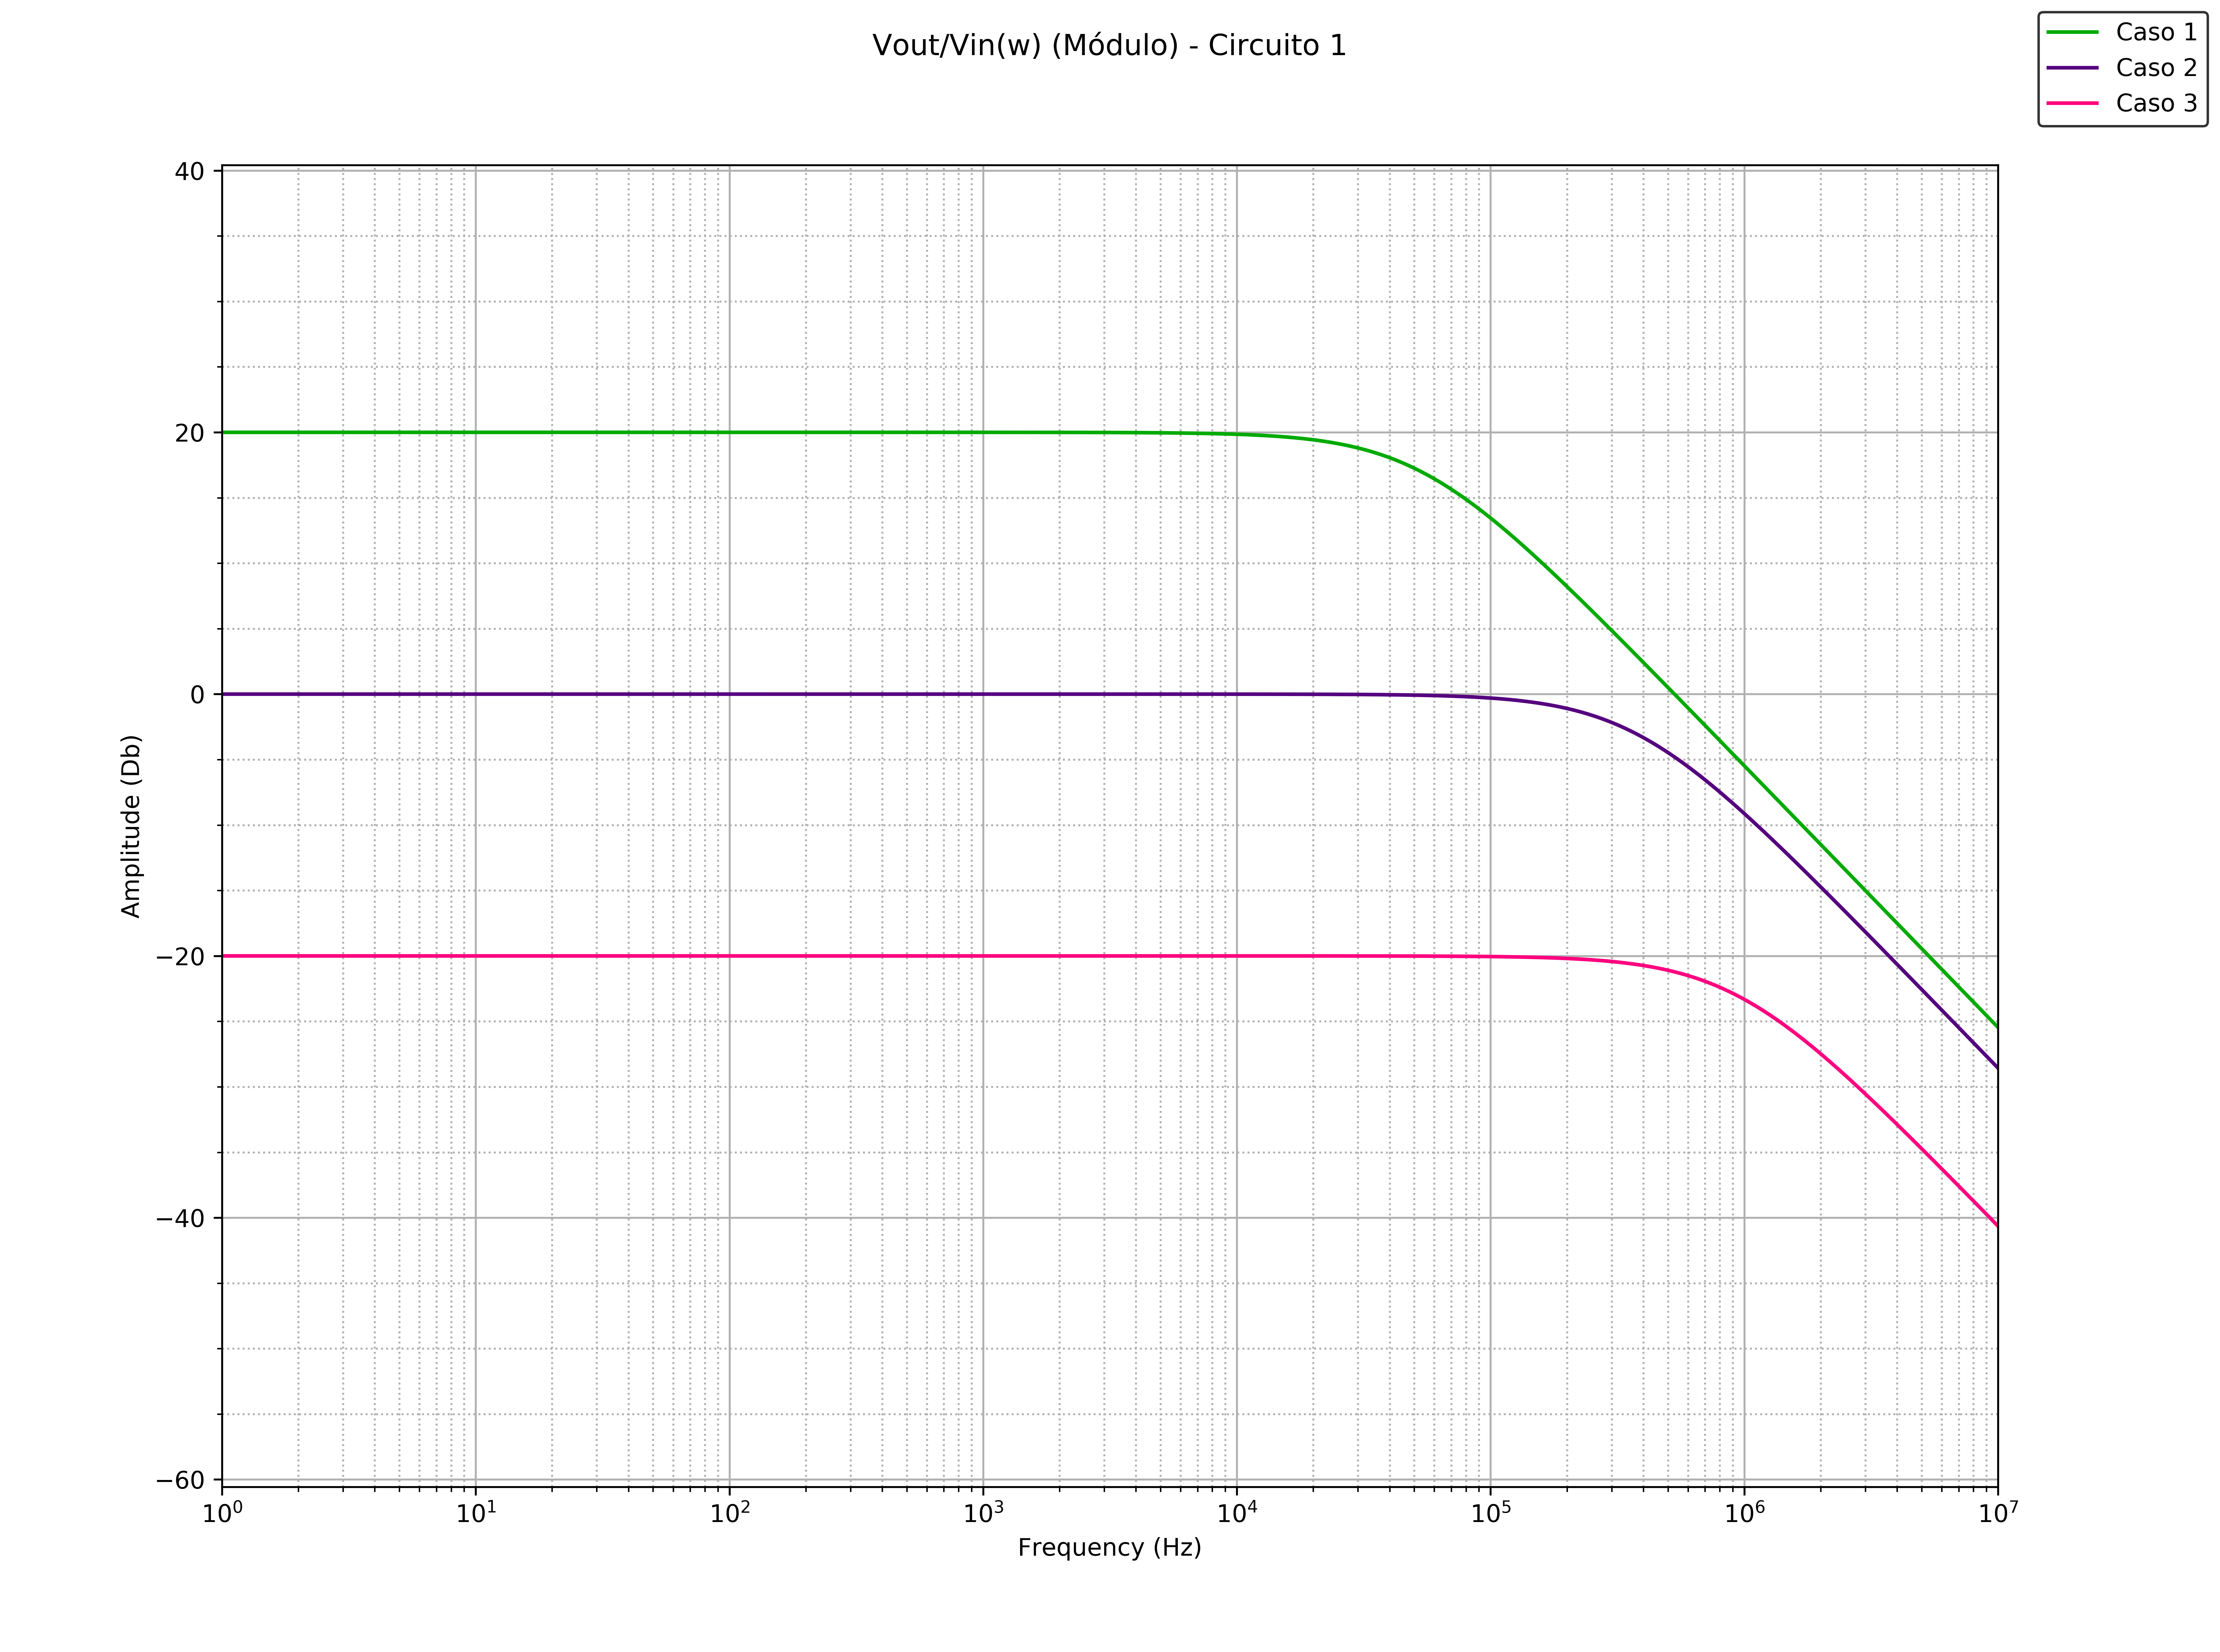
\includegraphics[scale=0.45]{../EJ1/00GRAFICOS/teoricos/circ1voviw.png}
	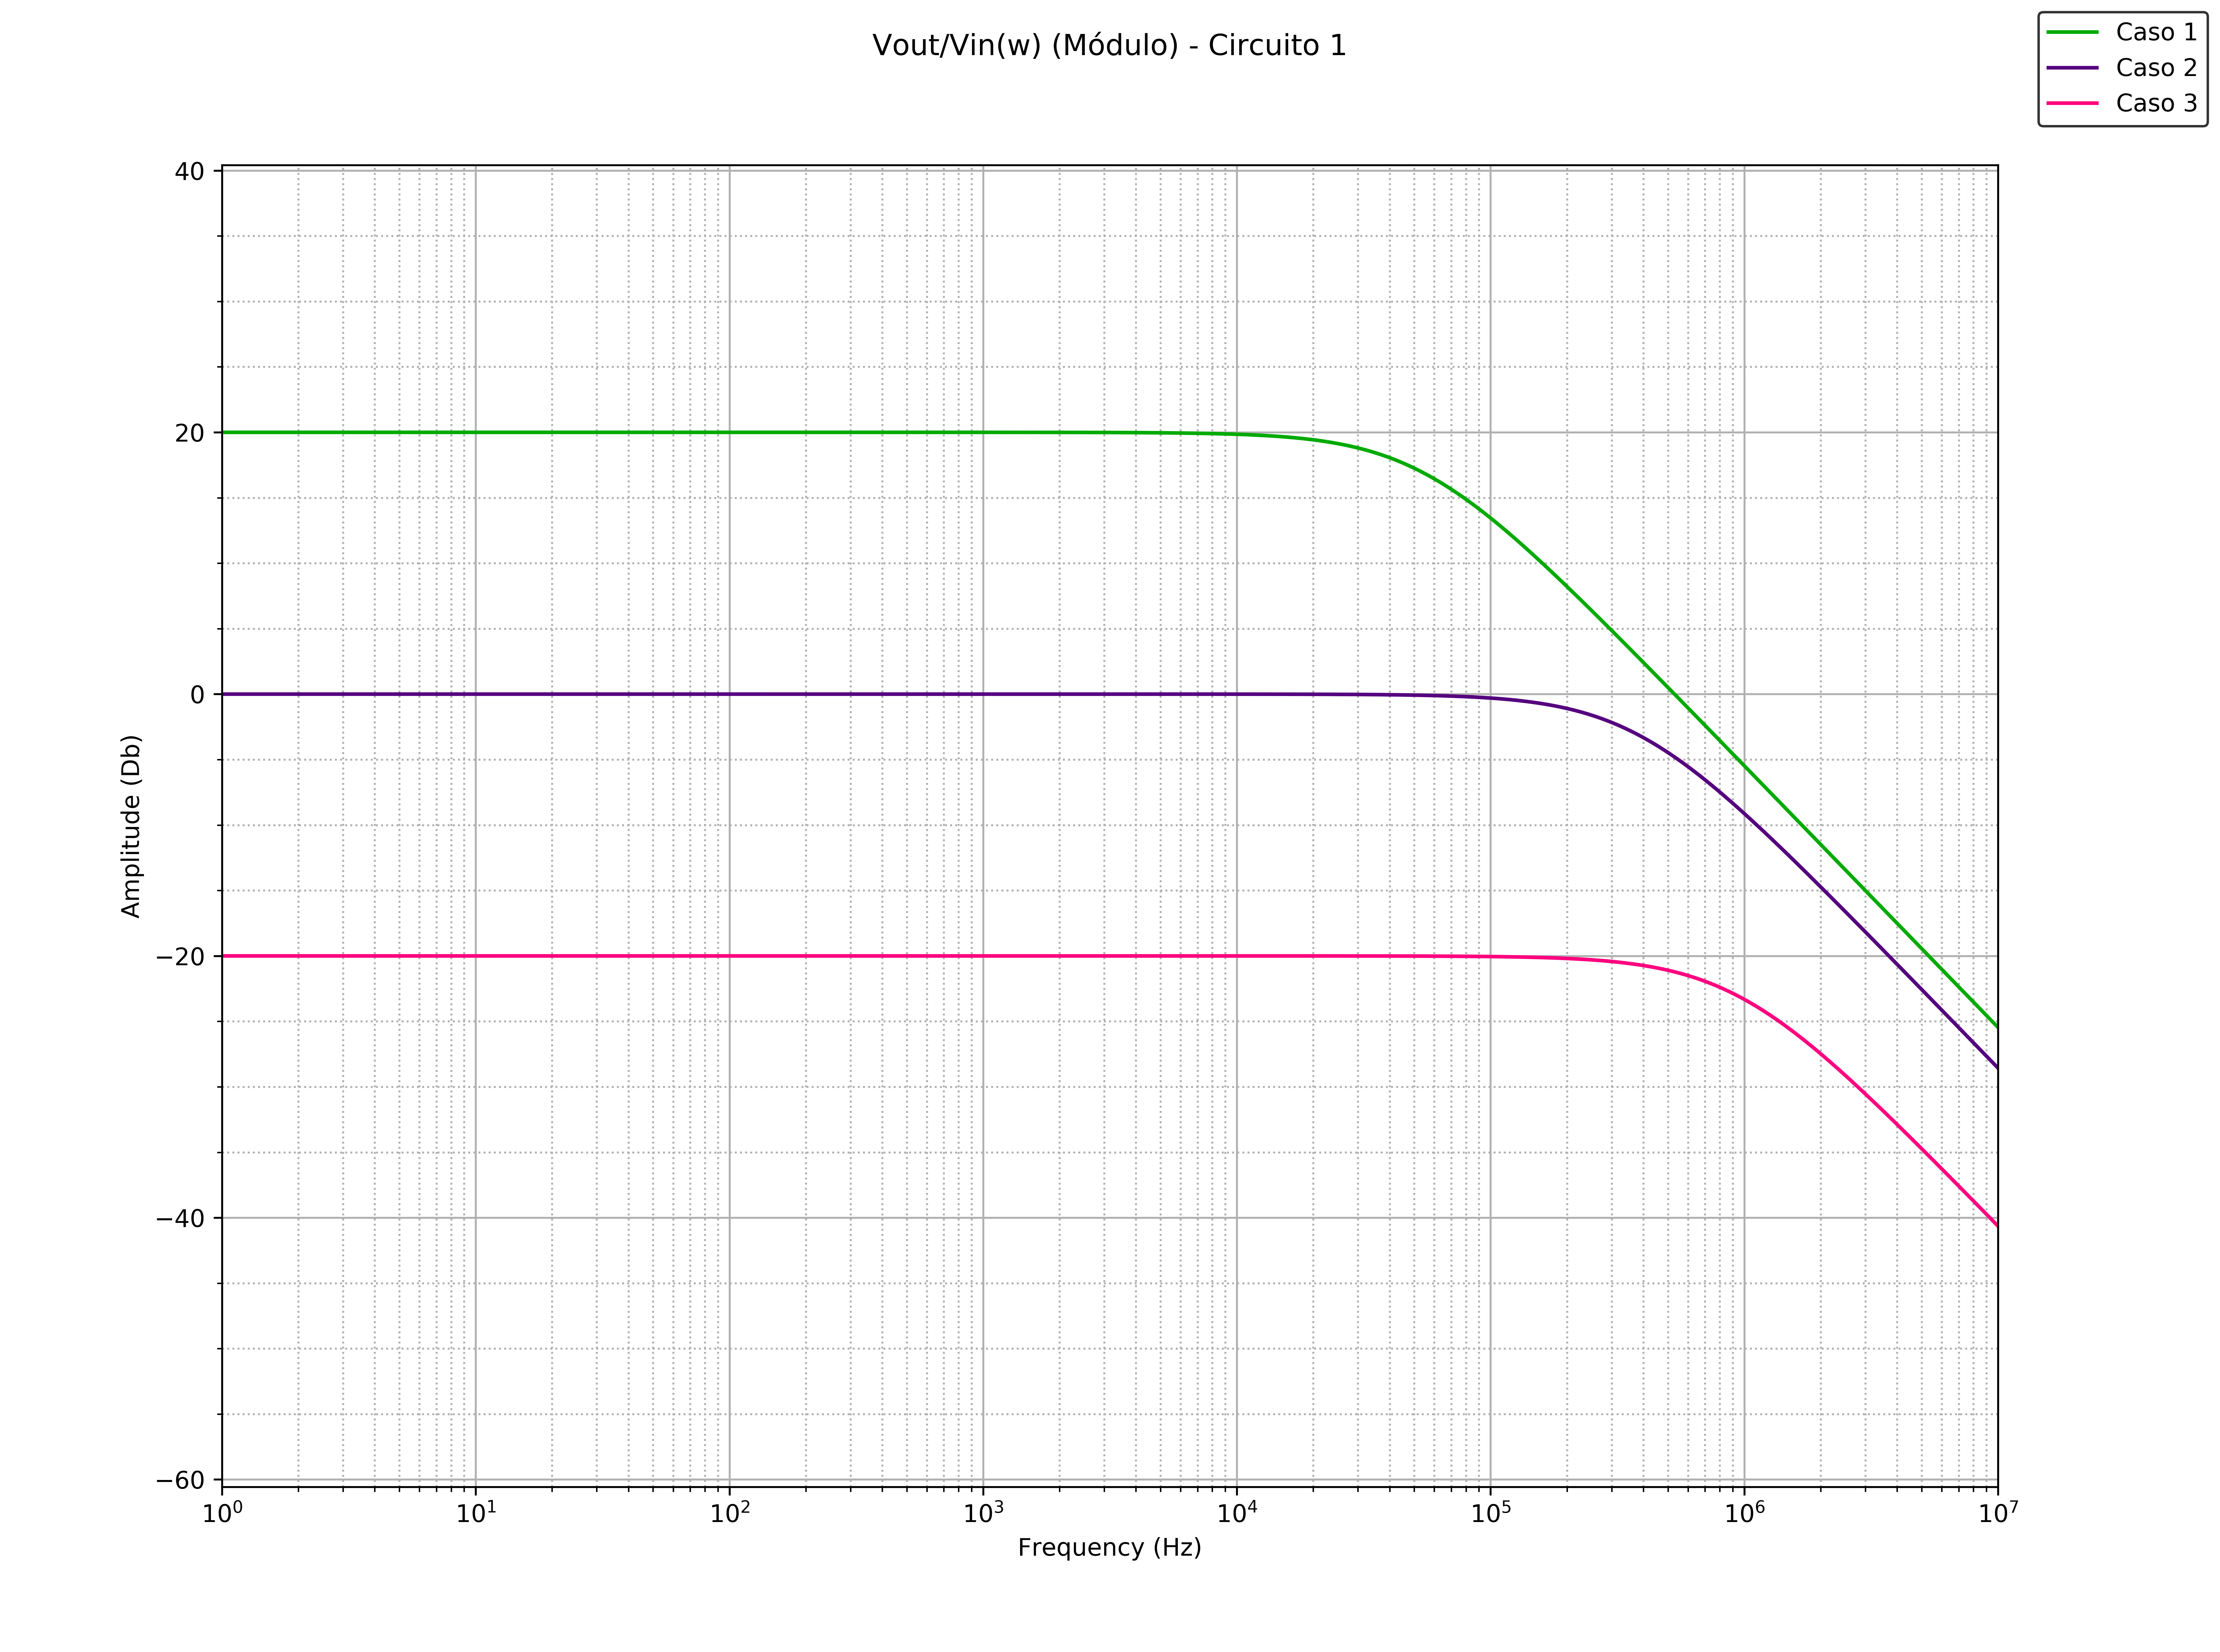
\includegraphics[width=10cm,height=10cm,keepaspectratio]{../EJ1/00GRAFICOS/teoricos/circ1voviw.png}
	\caption{Configuración inversora - Comparaci\'on te\'orica del m\'odulo de $V_{out}/V_{in}$ para los tres casos.}
	\label{c1voviTeoMod}
\end{figure}

\begin{figure}[H] %!ht
	\centering
	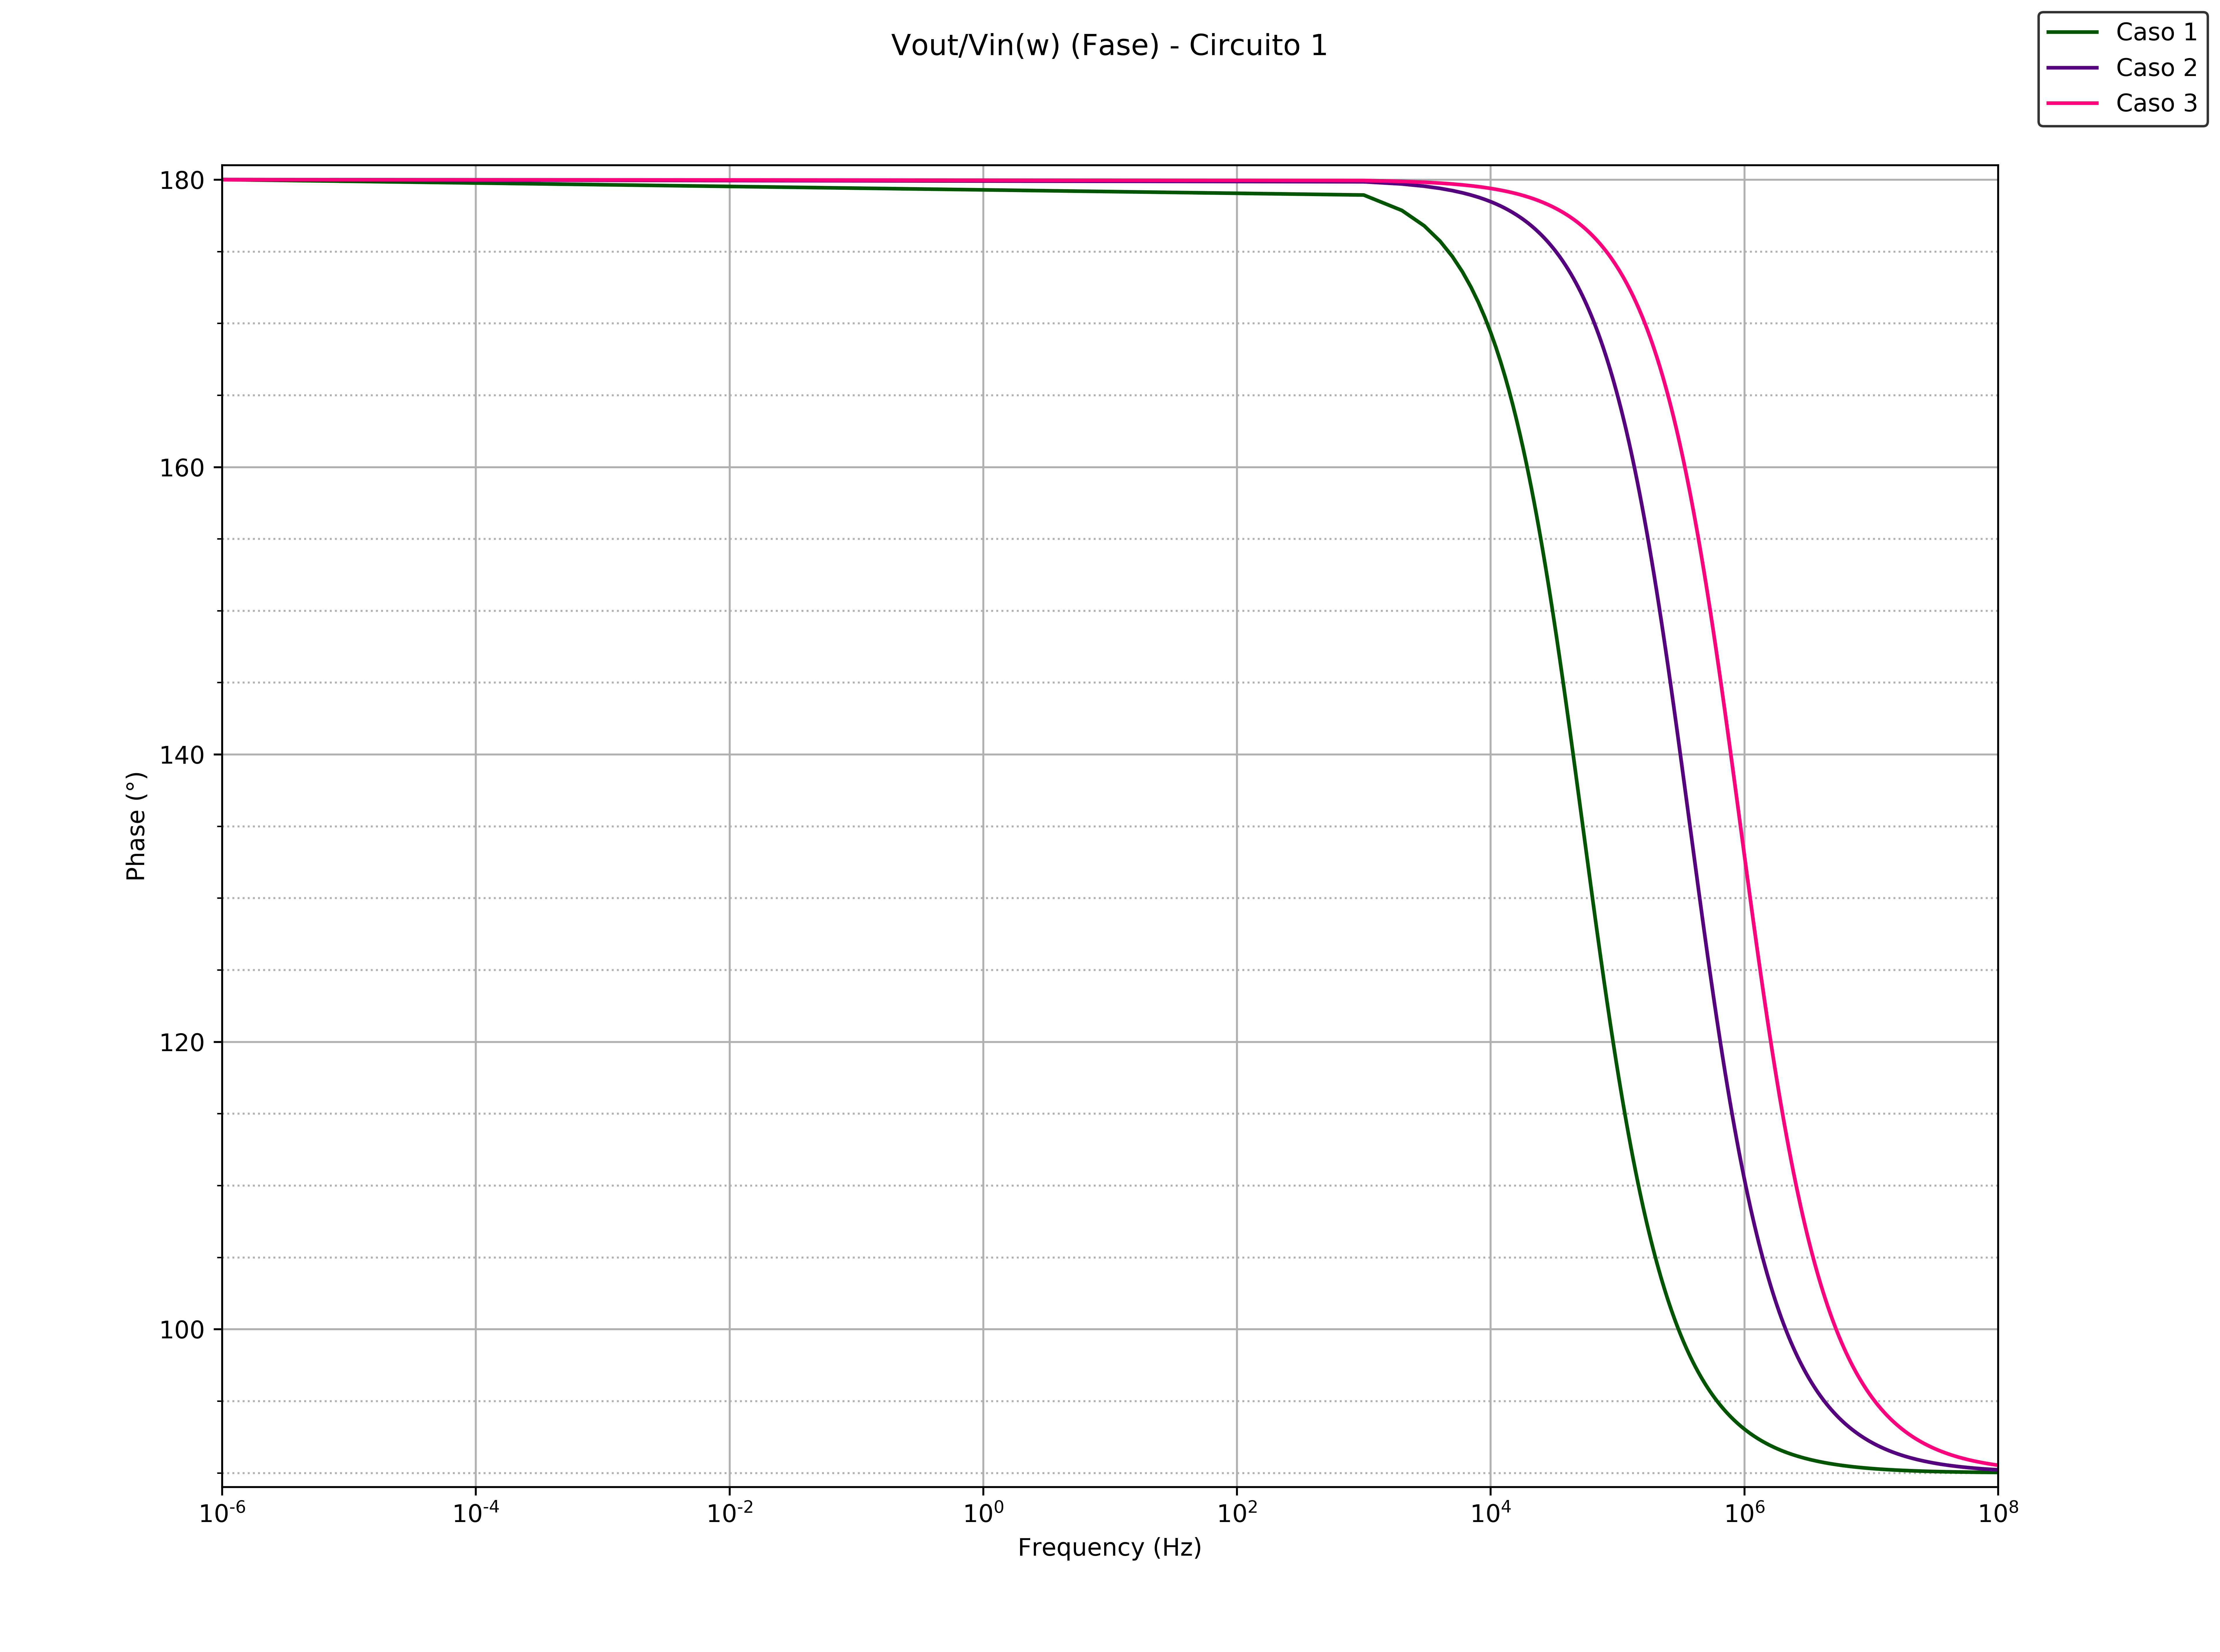
\includegraphics[width=10cm,height=10cm,keepaspectratio]{../EJ1/00GRAFICOS/teoricos/circ1vovifasew.png}
	\caption{Configuración inversora - Comparaci\'on te\'orica de la fase de $V_{out}/V_{in}$ para los tres casos.}
	\label{c1voviTeoPh}
\end{figure}

El gr\'afico \ref{c1voviTeoMod} permite ver una caracter\'istica importante que diferencia a los tres casos de resistencias para este circuito: la ganancia a bajas frecuencias. Las tres configuraciones corresponden a filtros pasabajos. Si bien aten\'uan a altas frecuencias, tienen comportamientos diferentes en las frecuencias bajas. Aqu\'el con resistencias para el caso 1 presenta una ganancia de 20dB, mientras que el del caso 3 aten\'ua 20 dB. El circuito del caso 2, por el contrario, no gana ni aten\'ua en frecuencias bajas.

%ANALIZAR AVOL FINITO . AVOL W ES LO QUE YA ESTA HECHO

\subsubsection*{Configuraci\'on no inversora}

\begin{figure}[H] %!ht
\centering
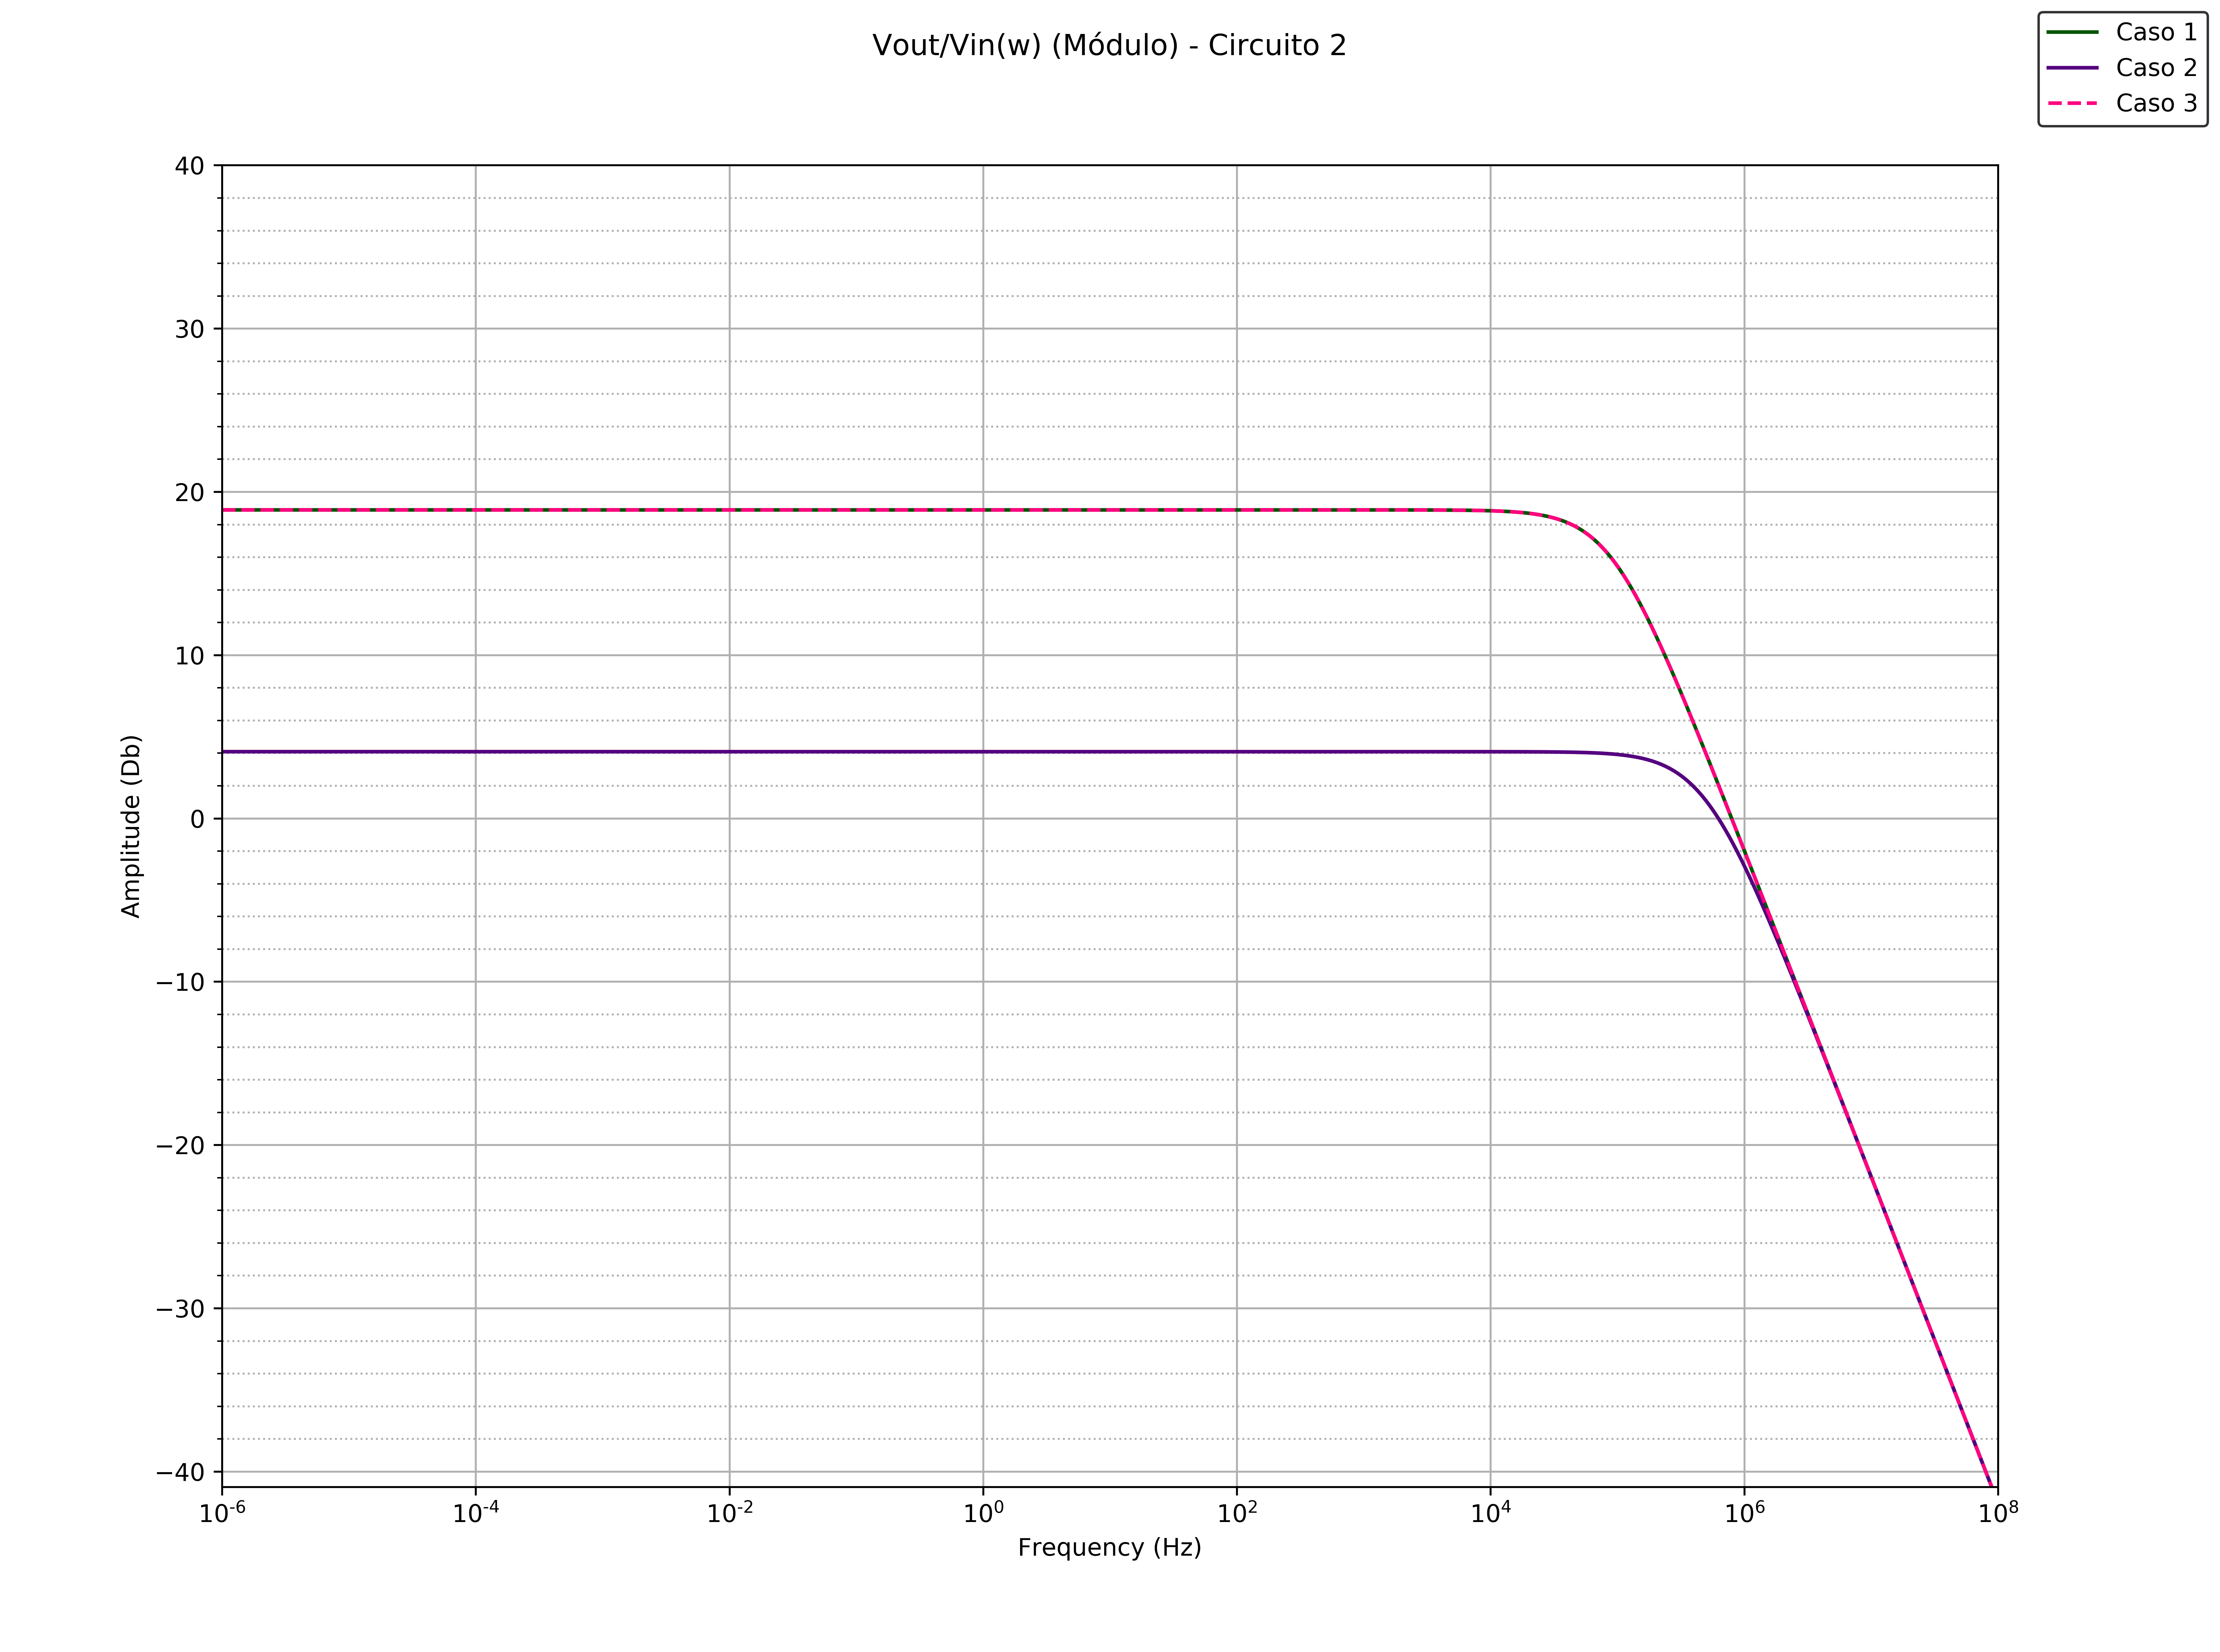
\includegraphics[width=10cm,height=10cm,keepaspectratio]{../EJ1/00GRAFICOS/teoricos/circ2voviw.png}
\caption{Configuración no inversora - Comparaci\'on te\'orica del m\'odulo de$V_{out}/V_{in}$ de los tres casos.}
\label{c2voviTeoMod}
\end{figure}

\begin{figure}[H] %!ht
\centering
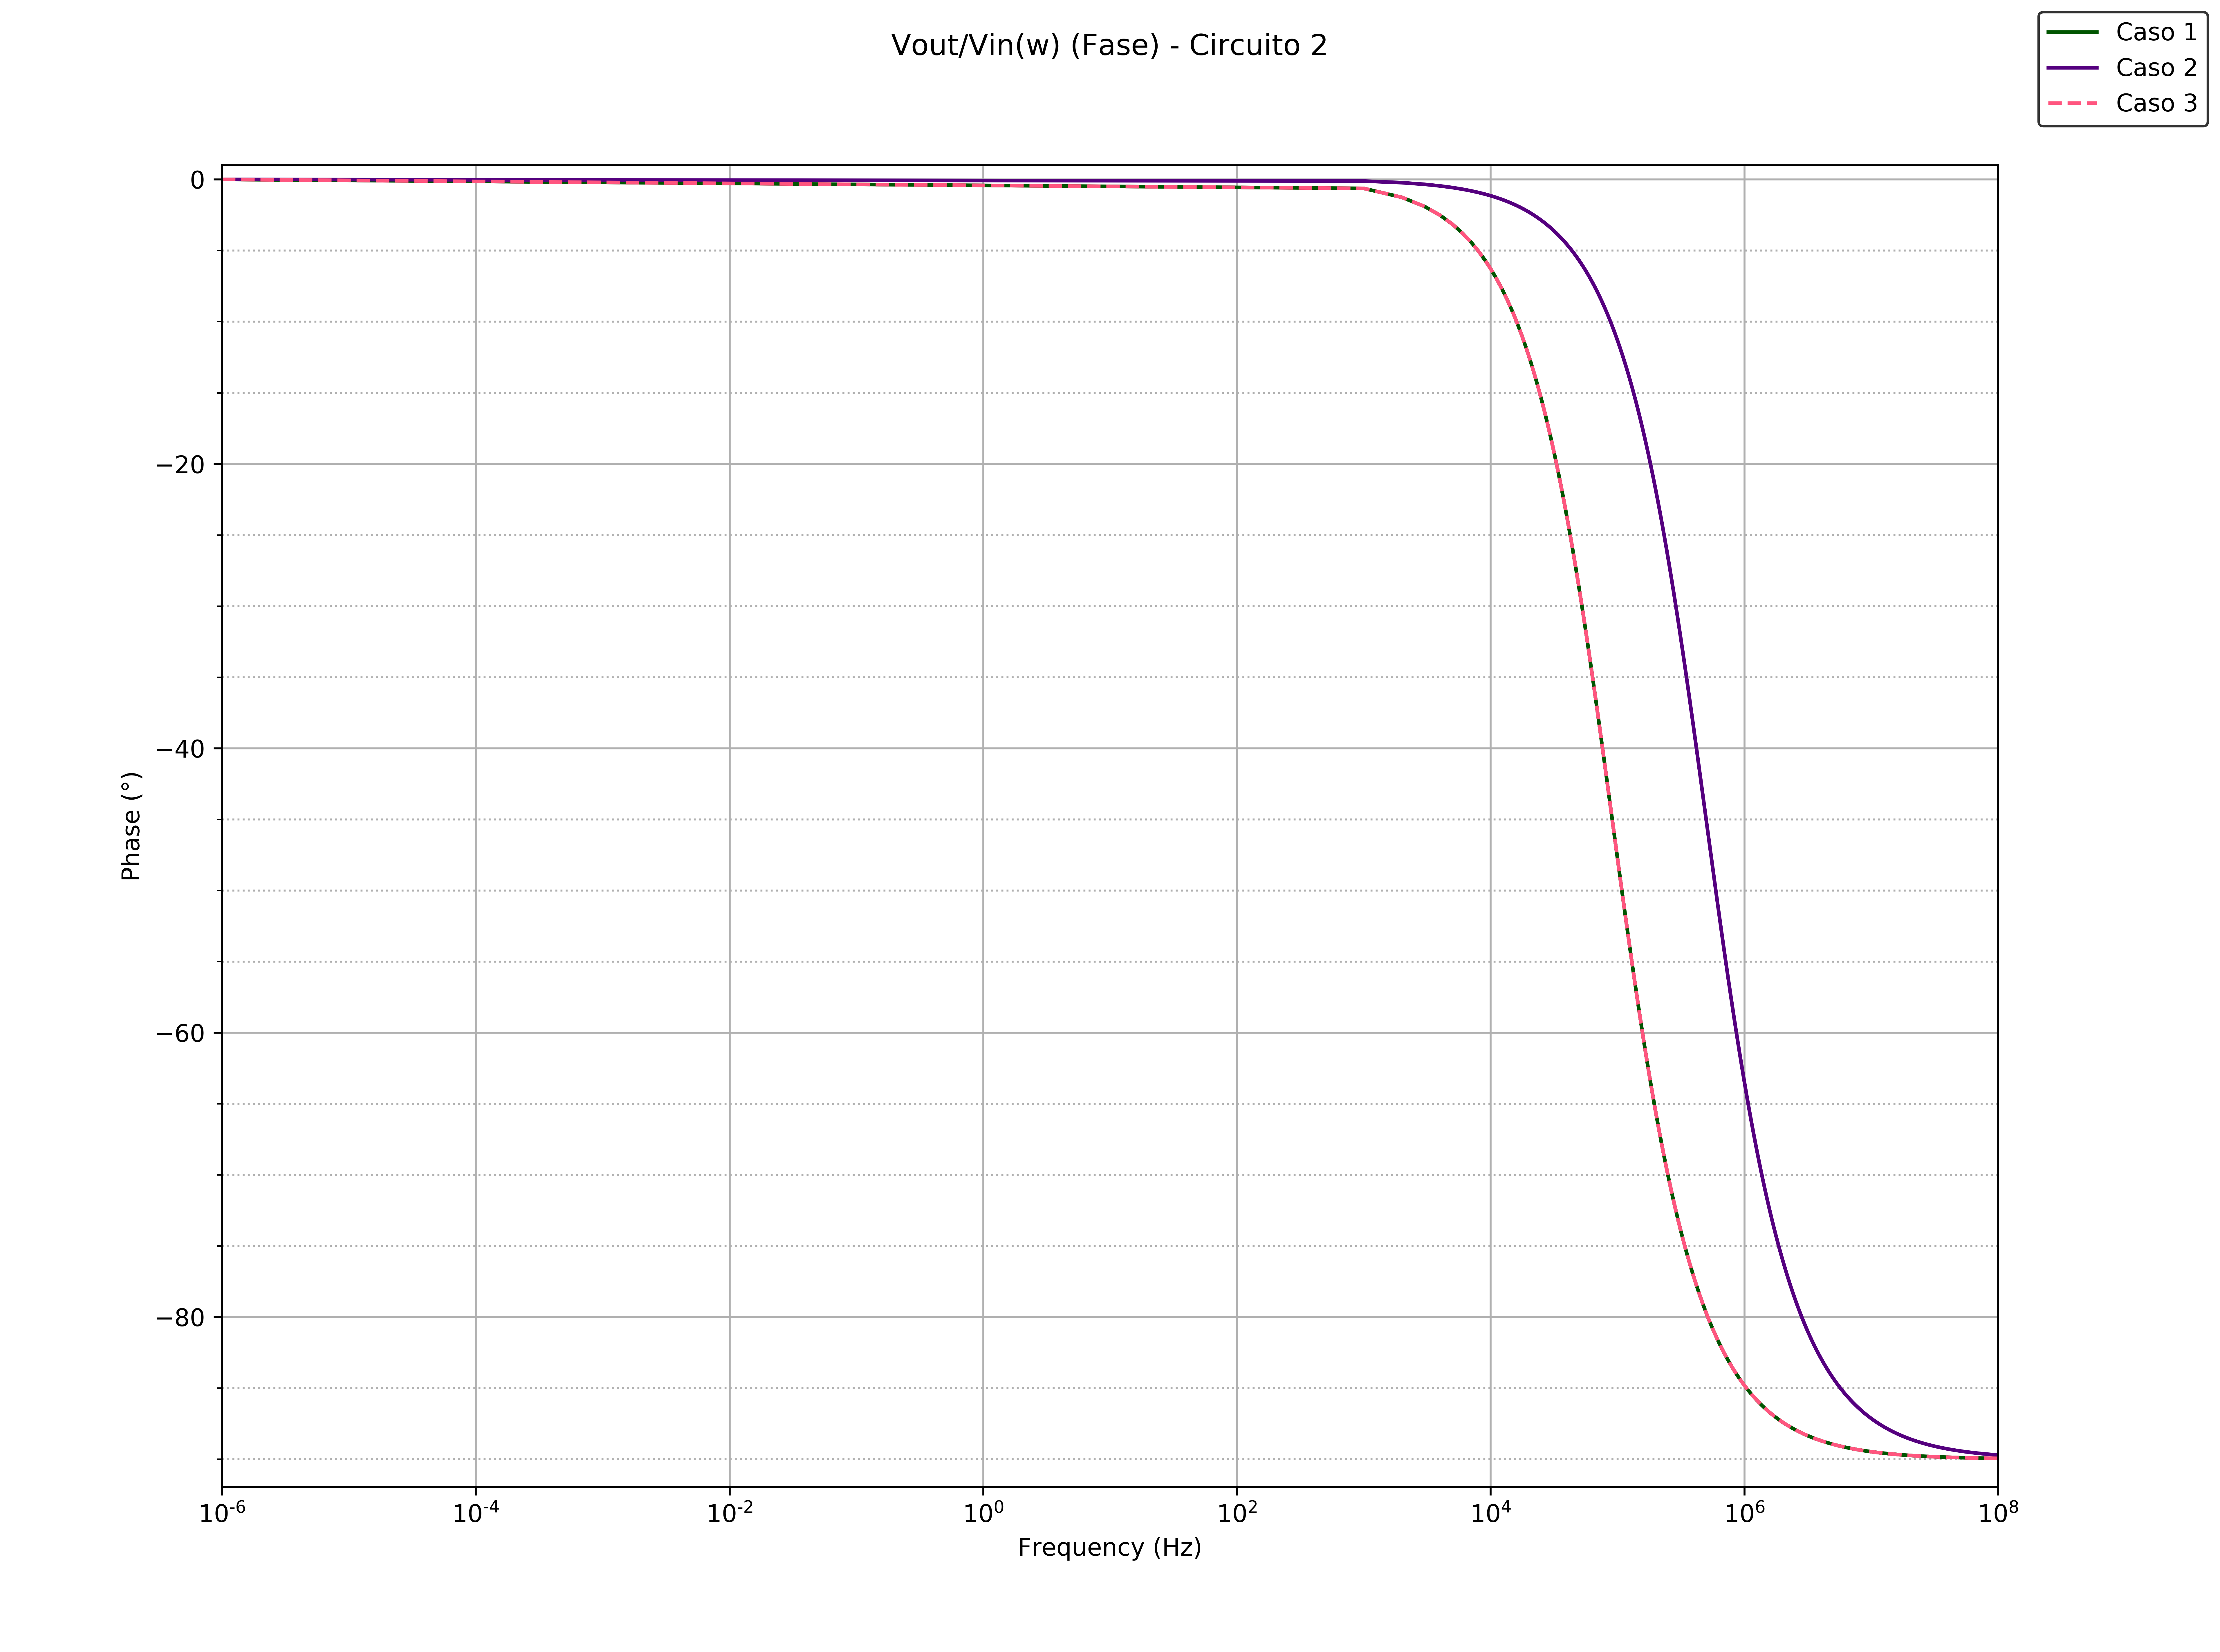
\includegraphics[width=10cm,height=10cm,keepaspectratio]{../EJ1/00GRAFICOS/teoricos/circ2vovifasew.png}
\caption{Configuración no inversora - Comparaci\'on te\'orica de la fase de $V_{out}/V_{in}$ de los tres casos.}
\label{c2voviTeoPh}
\end{figure}






\subsubsection{Mediciones y resultados obtenidos} %%%%%%%

\subsubsection*{Configuraci\'on inversora}
Se simul\'o y se midi\'o la ganancia para los tres casos del circuito \ref{c1} y a continuacio\'on se puede ver la diferencia entre sus resultados y los de las ecuaciones \ref{c1c1vovi}, \ref{c1c2vovi} y \ref{c1c3vovi}; correspondientes a la ganancia calculada de forma te\'orica y considerando al amplificador operacional como ideal.

\begin{figure}[H] %!ht
	\centering
	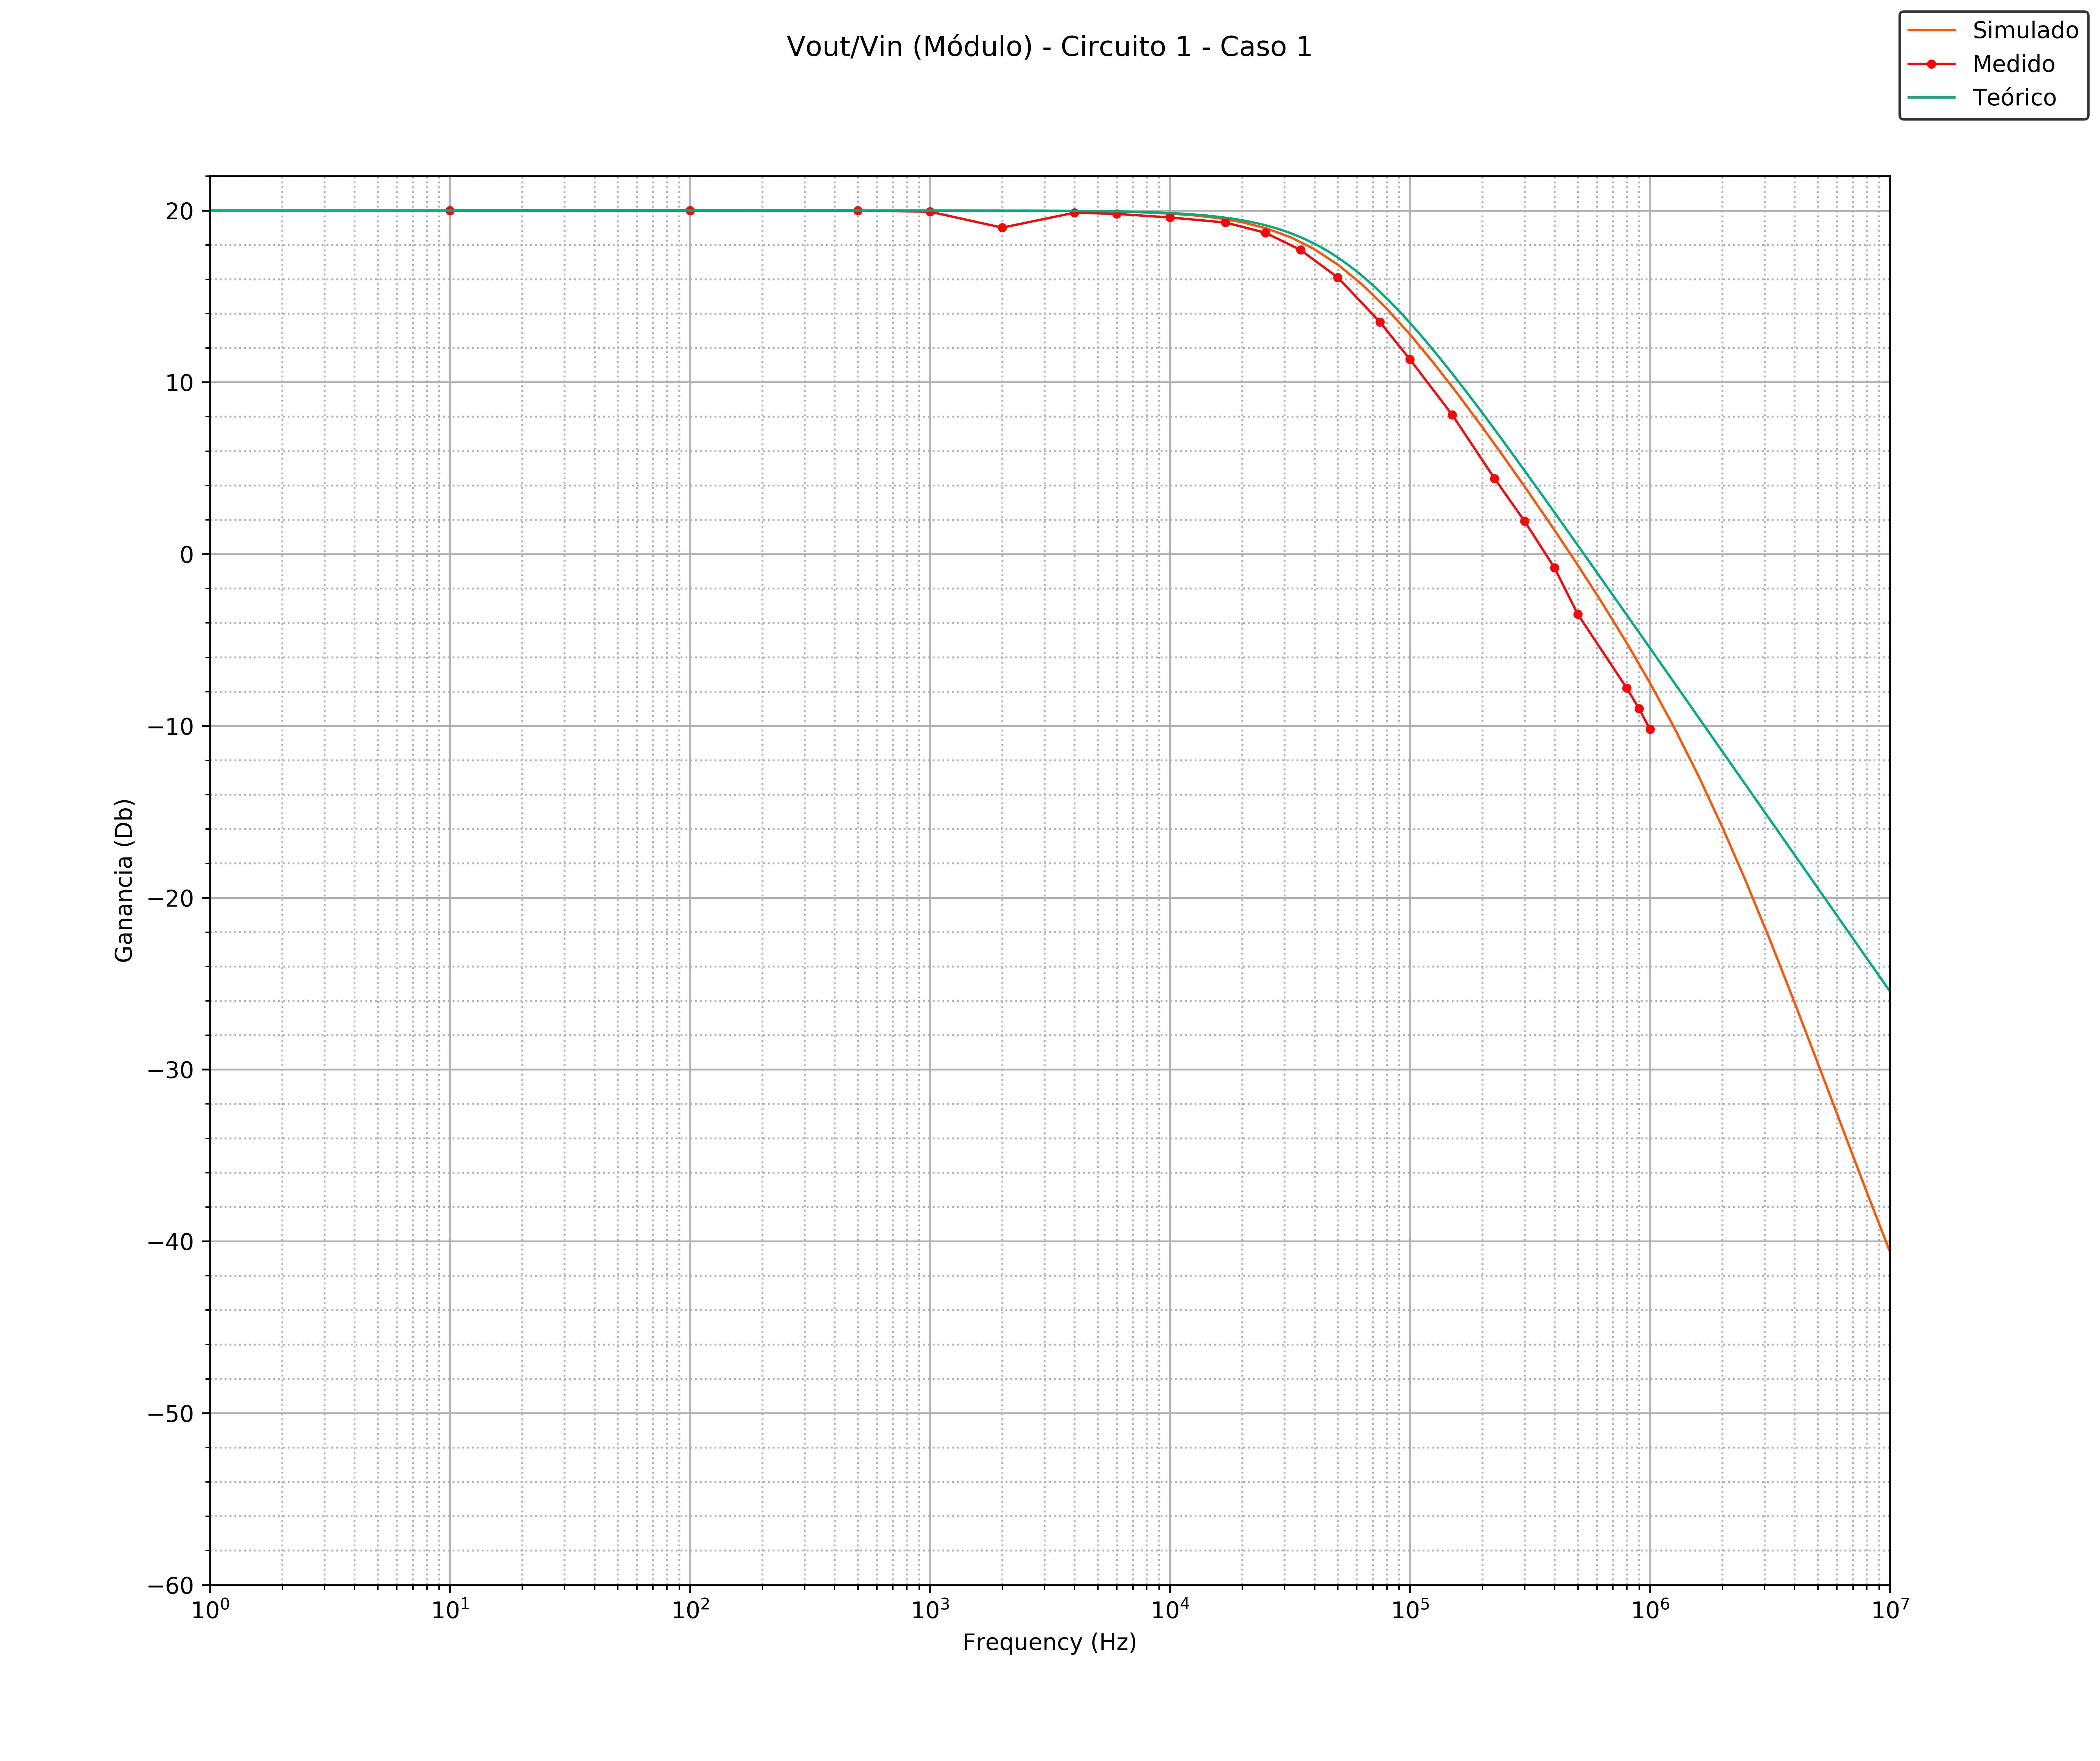
\includegraphics[width=10cm,height=10cm,keepaspectratio]{../EJ1/00GRAFICOS/c1c1/c1c1voviMod.png}
	\caption{Configuración inversora -  Caso 1 - Módulo de $V_{out}/V_{in}$}
	\label{c1c1voviM}
\end{figure}

\begin{figure}[H] %!ht
	\centering
	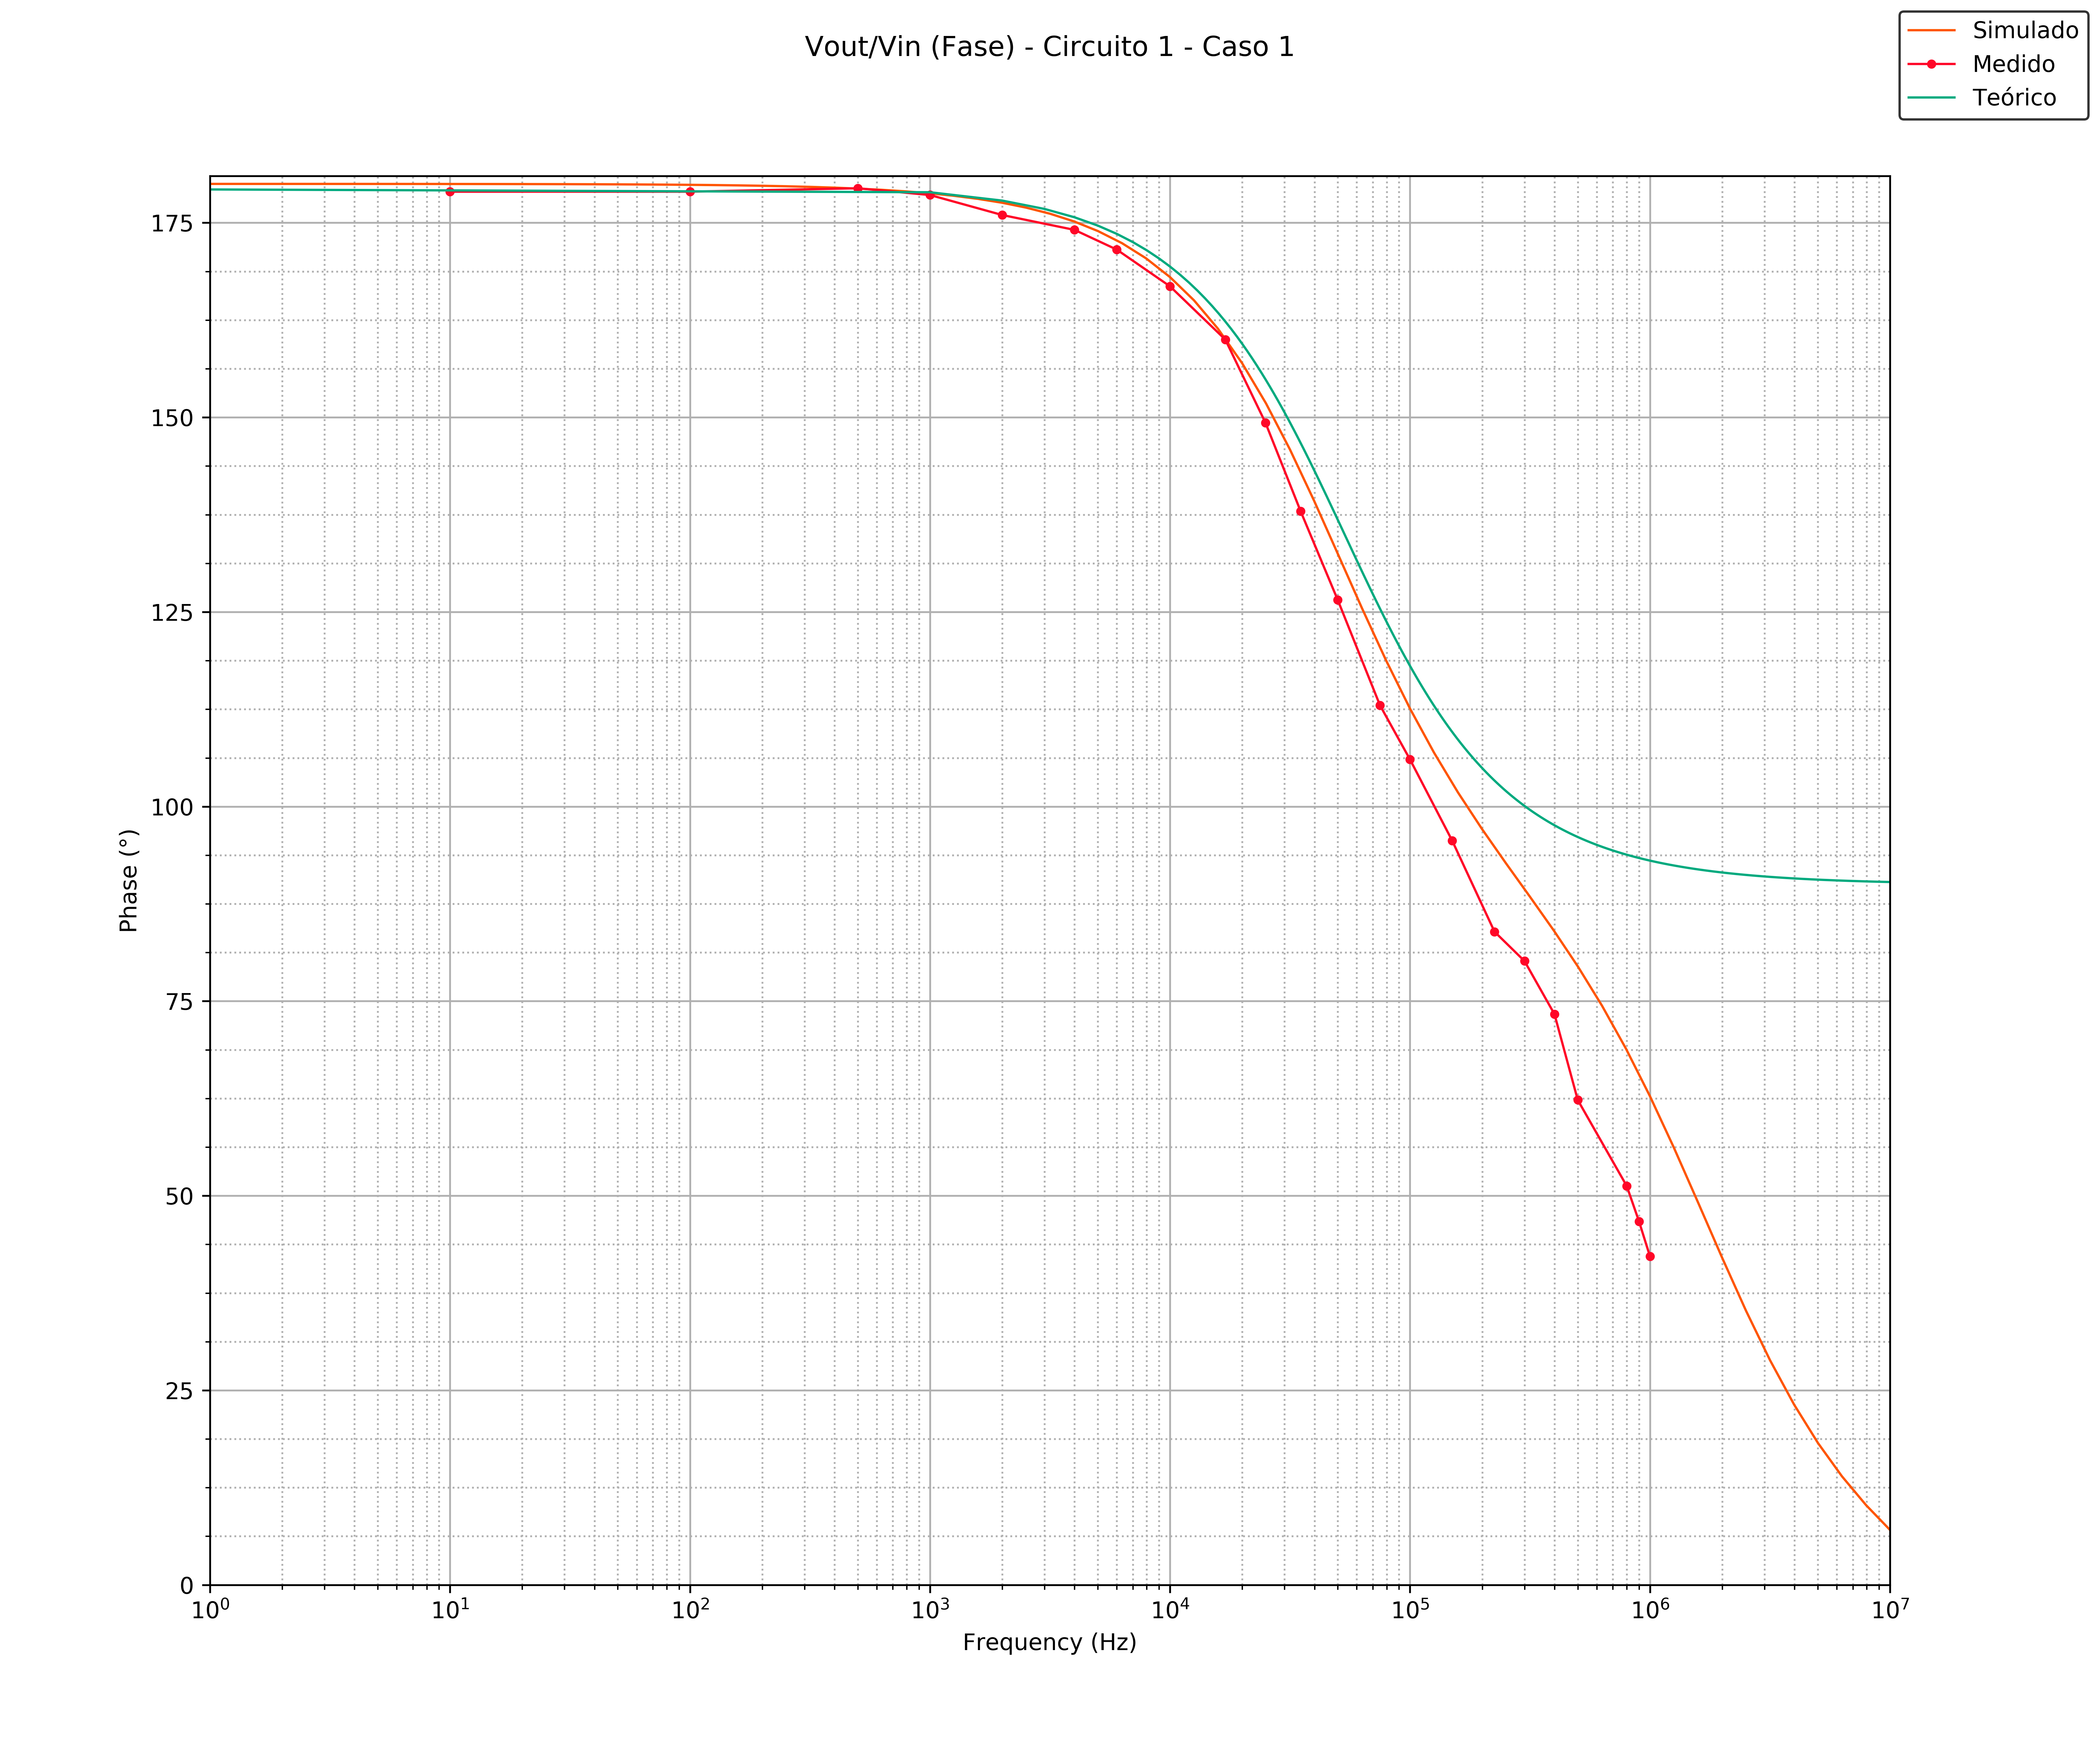
\includegraphics[width=10cm,height=10cm,keepaspectratio]{../EJ1/00GRAFICOS/c1c1/c1c1voviFASE.png}
	\caption{Configuración inversora - Caso 1 - Fase de $V_{out}/V_{in}$}
	\label{c1c1voviP}
\end{figure}

\begin{figure}[H] %!ht
	\centering
	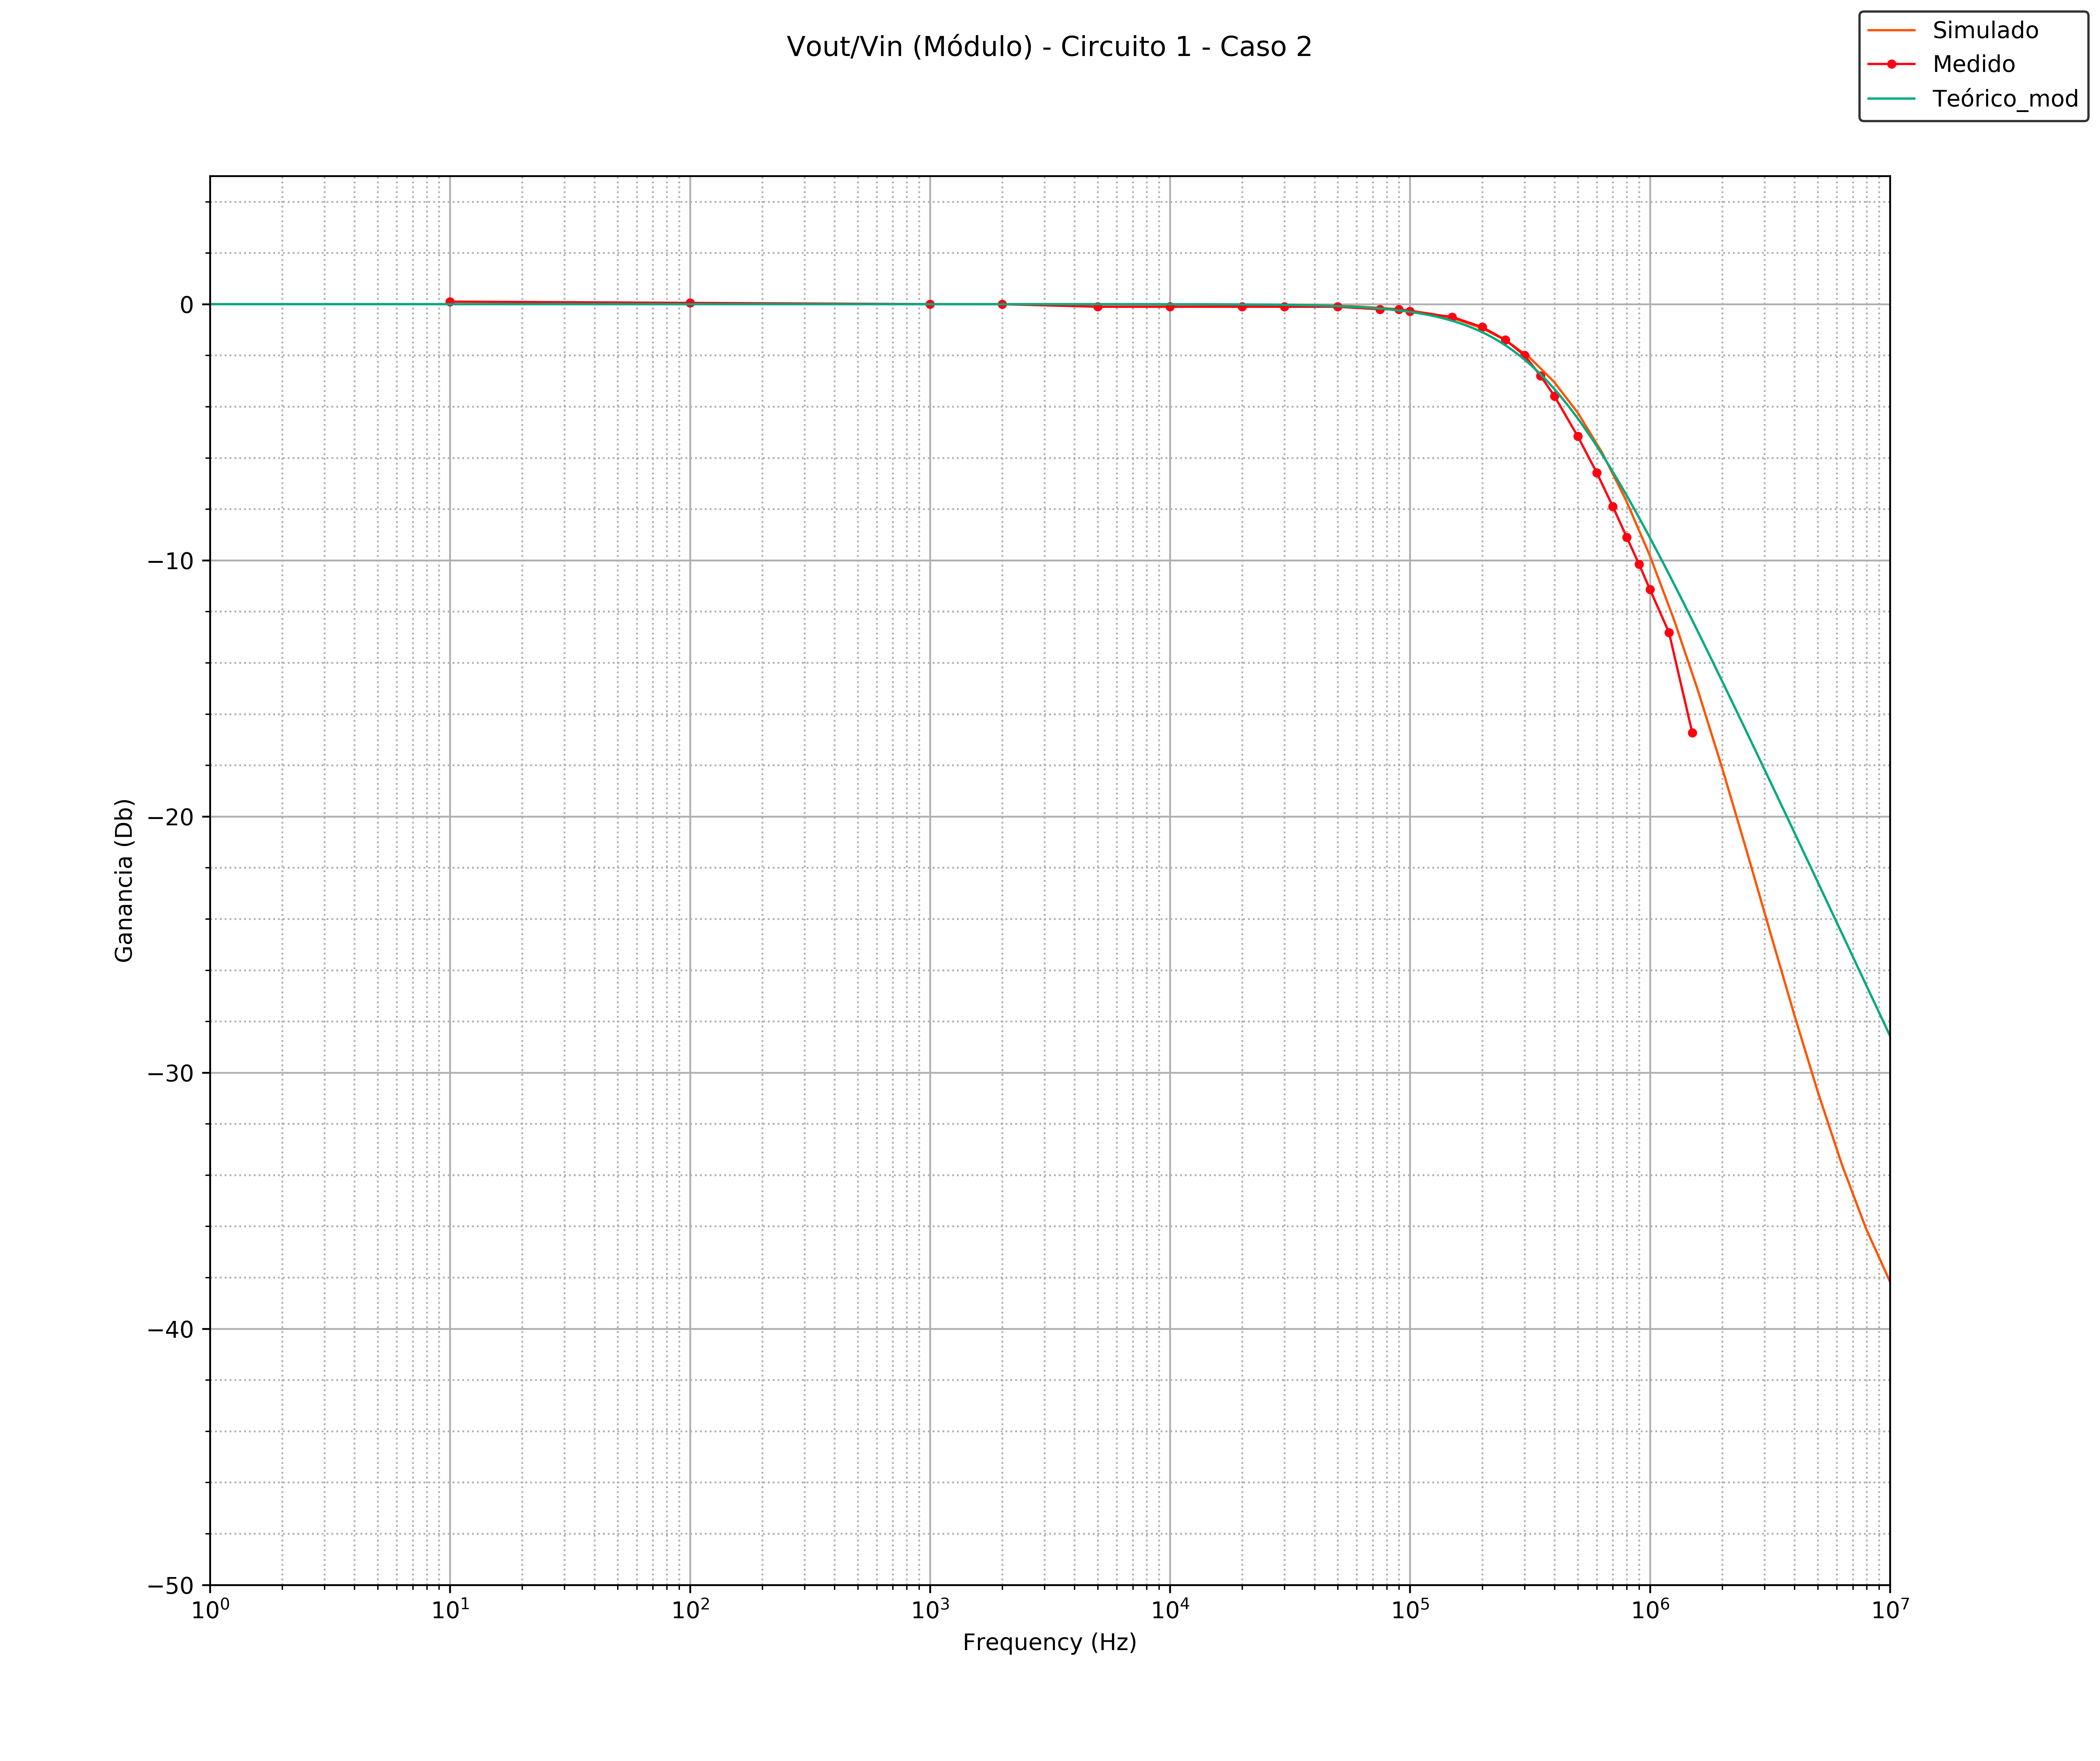
\includegraphics[width=10cm,height=10cm,keepaspectratio]{../EJ1/00GRAFICOS/c1c2/c1c2voviMod.png}
	\caption{Configuración inversora - Caso 2 - Módulo de $V_{out}/V_{in}$}
	\label{c1c2voviM}
\end{figure}

\begin{figure}[H] %!ht
	\centering
	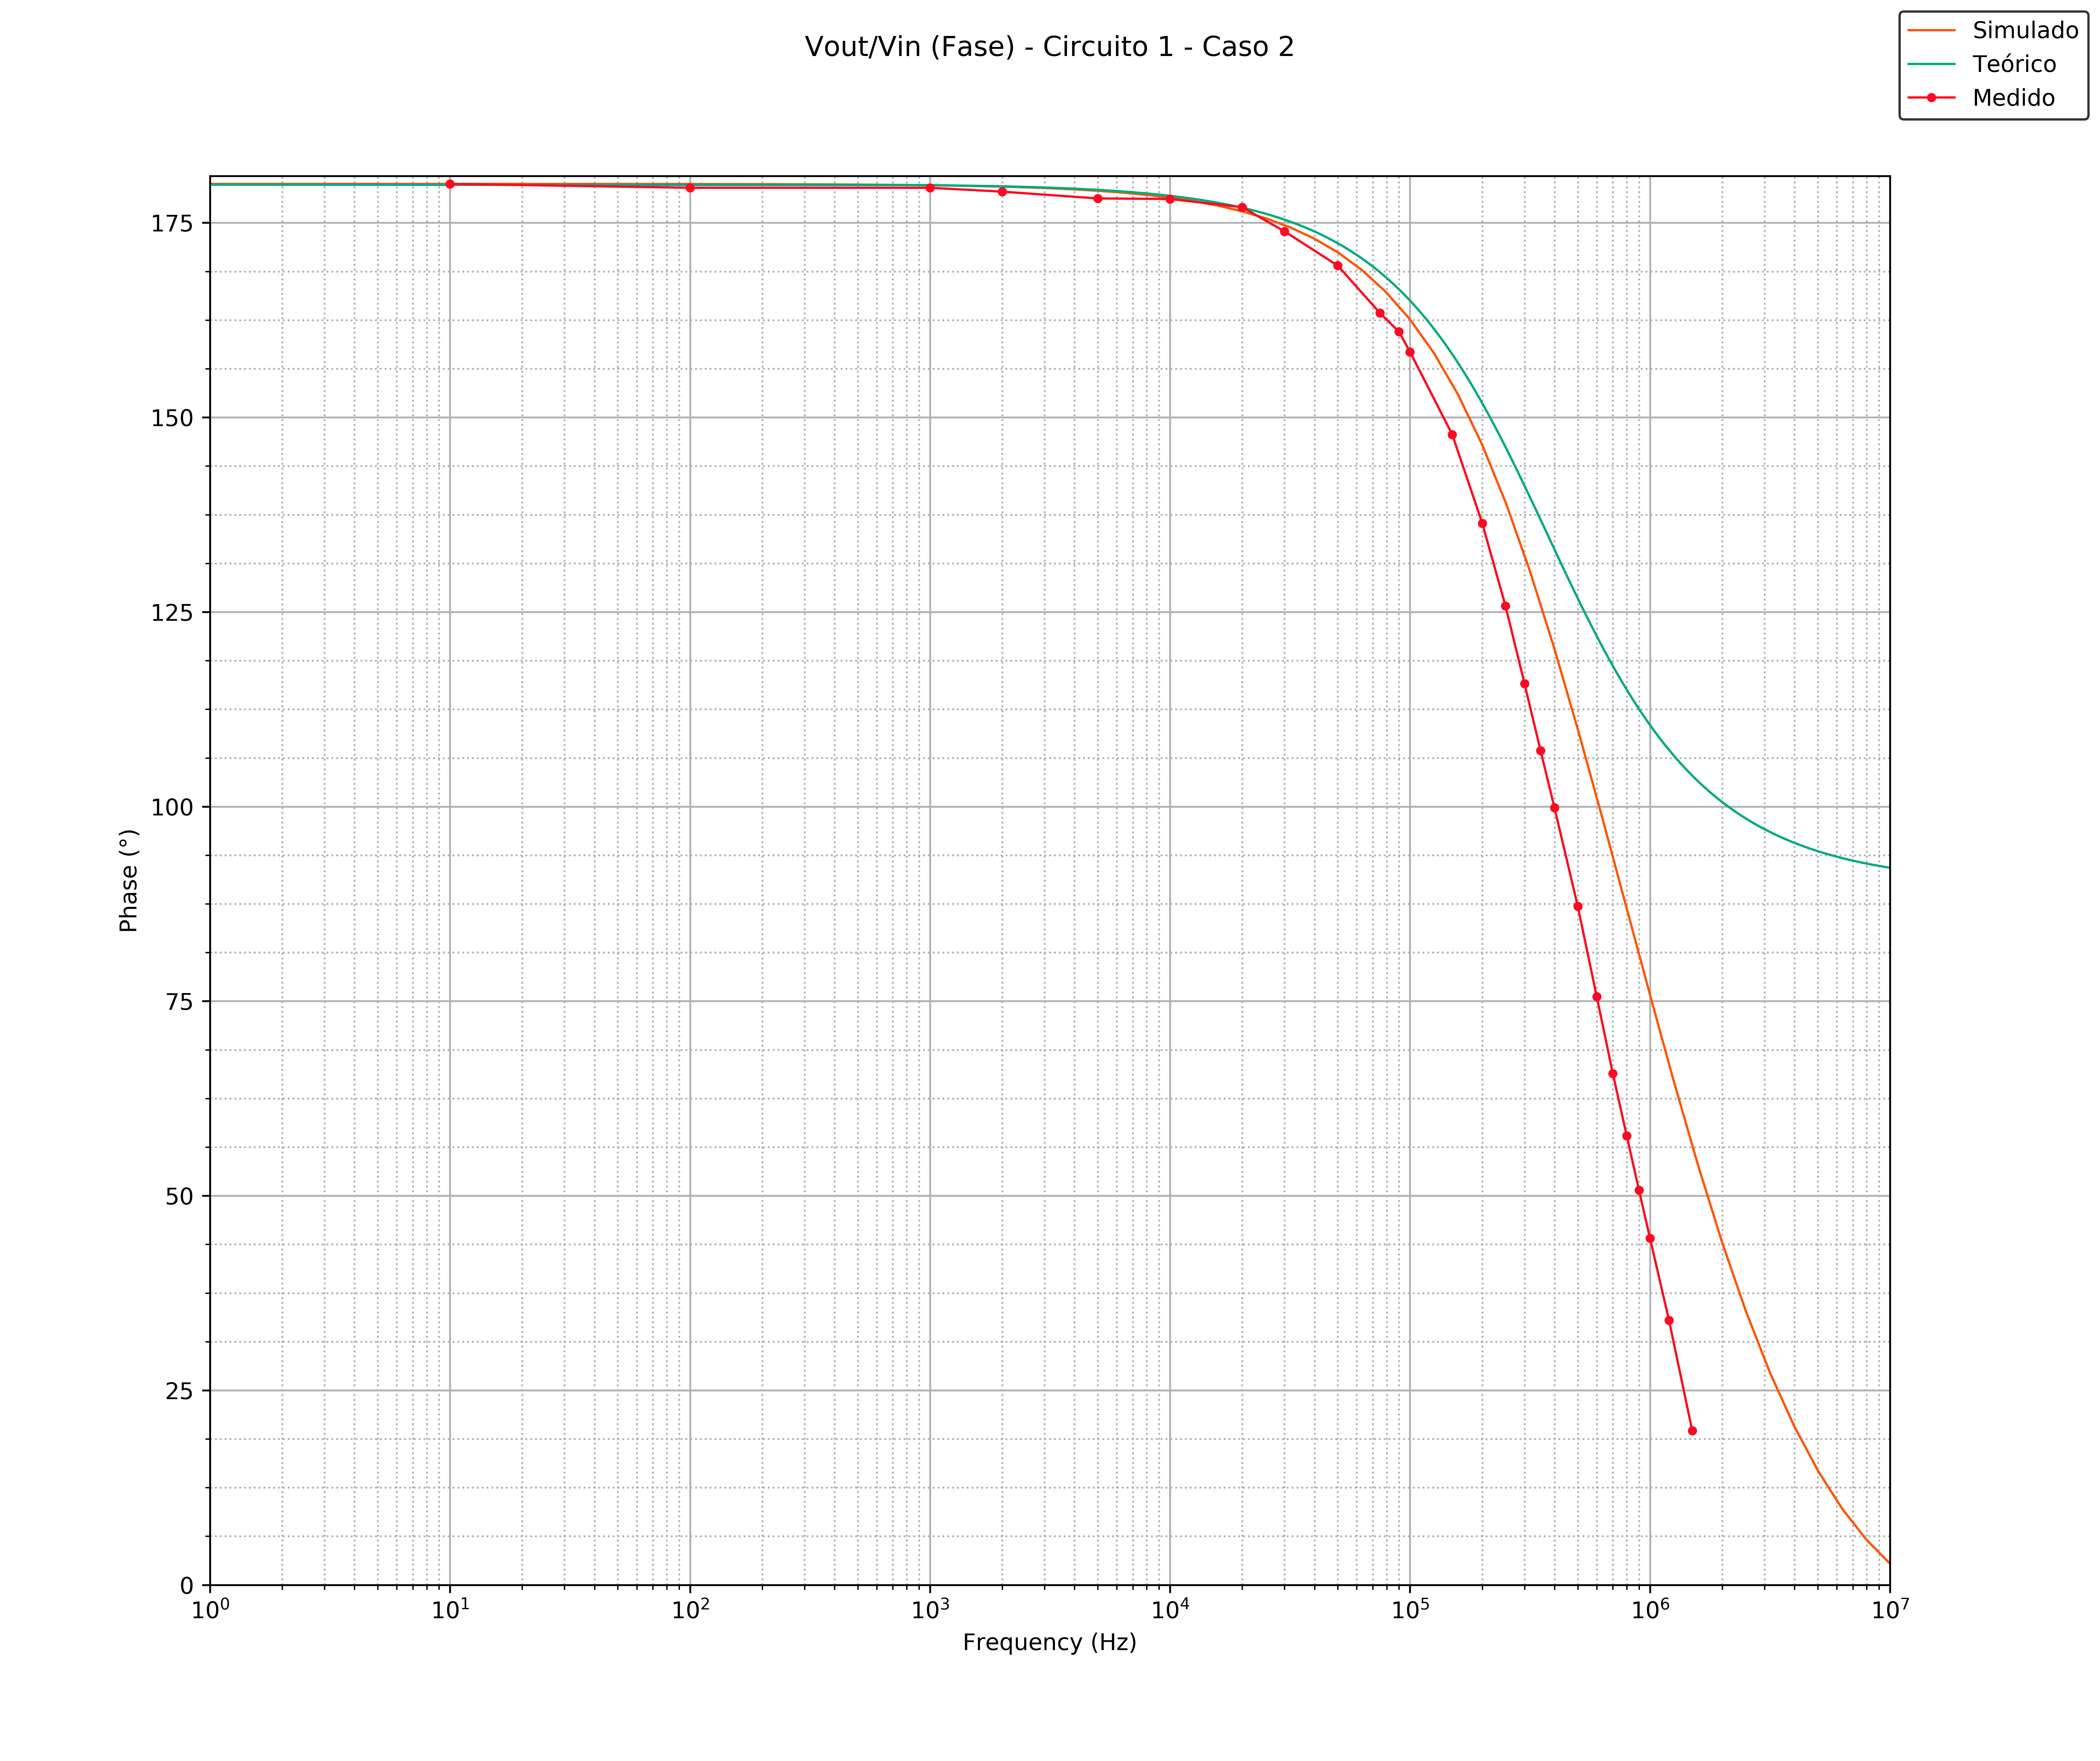
\includegraphics[width=10cm,height=10cm,keepaspectratio]{../EJ1/00GRAFICOS/c1c2/c1c2voviFASE.png}
	\caption{Configuración inversora - Caso 2 - Fase de $V_{out}/V_{in}$ }
	\label{c1c2voviP}
\end{figure}

\begin{figure}[H] %!ht
	\centering
	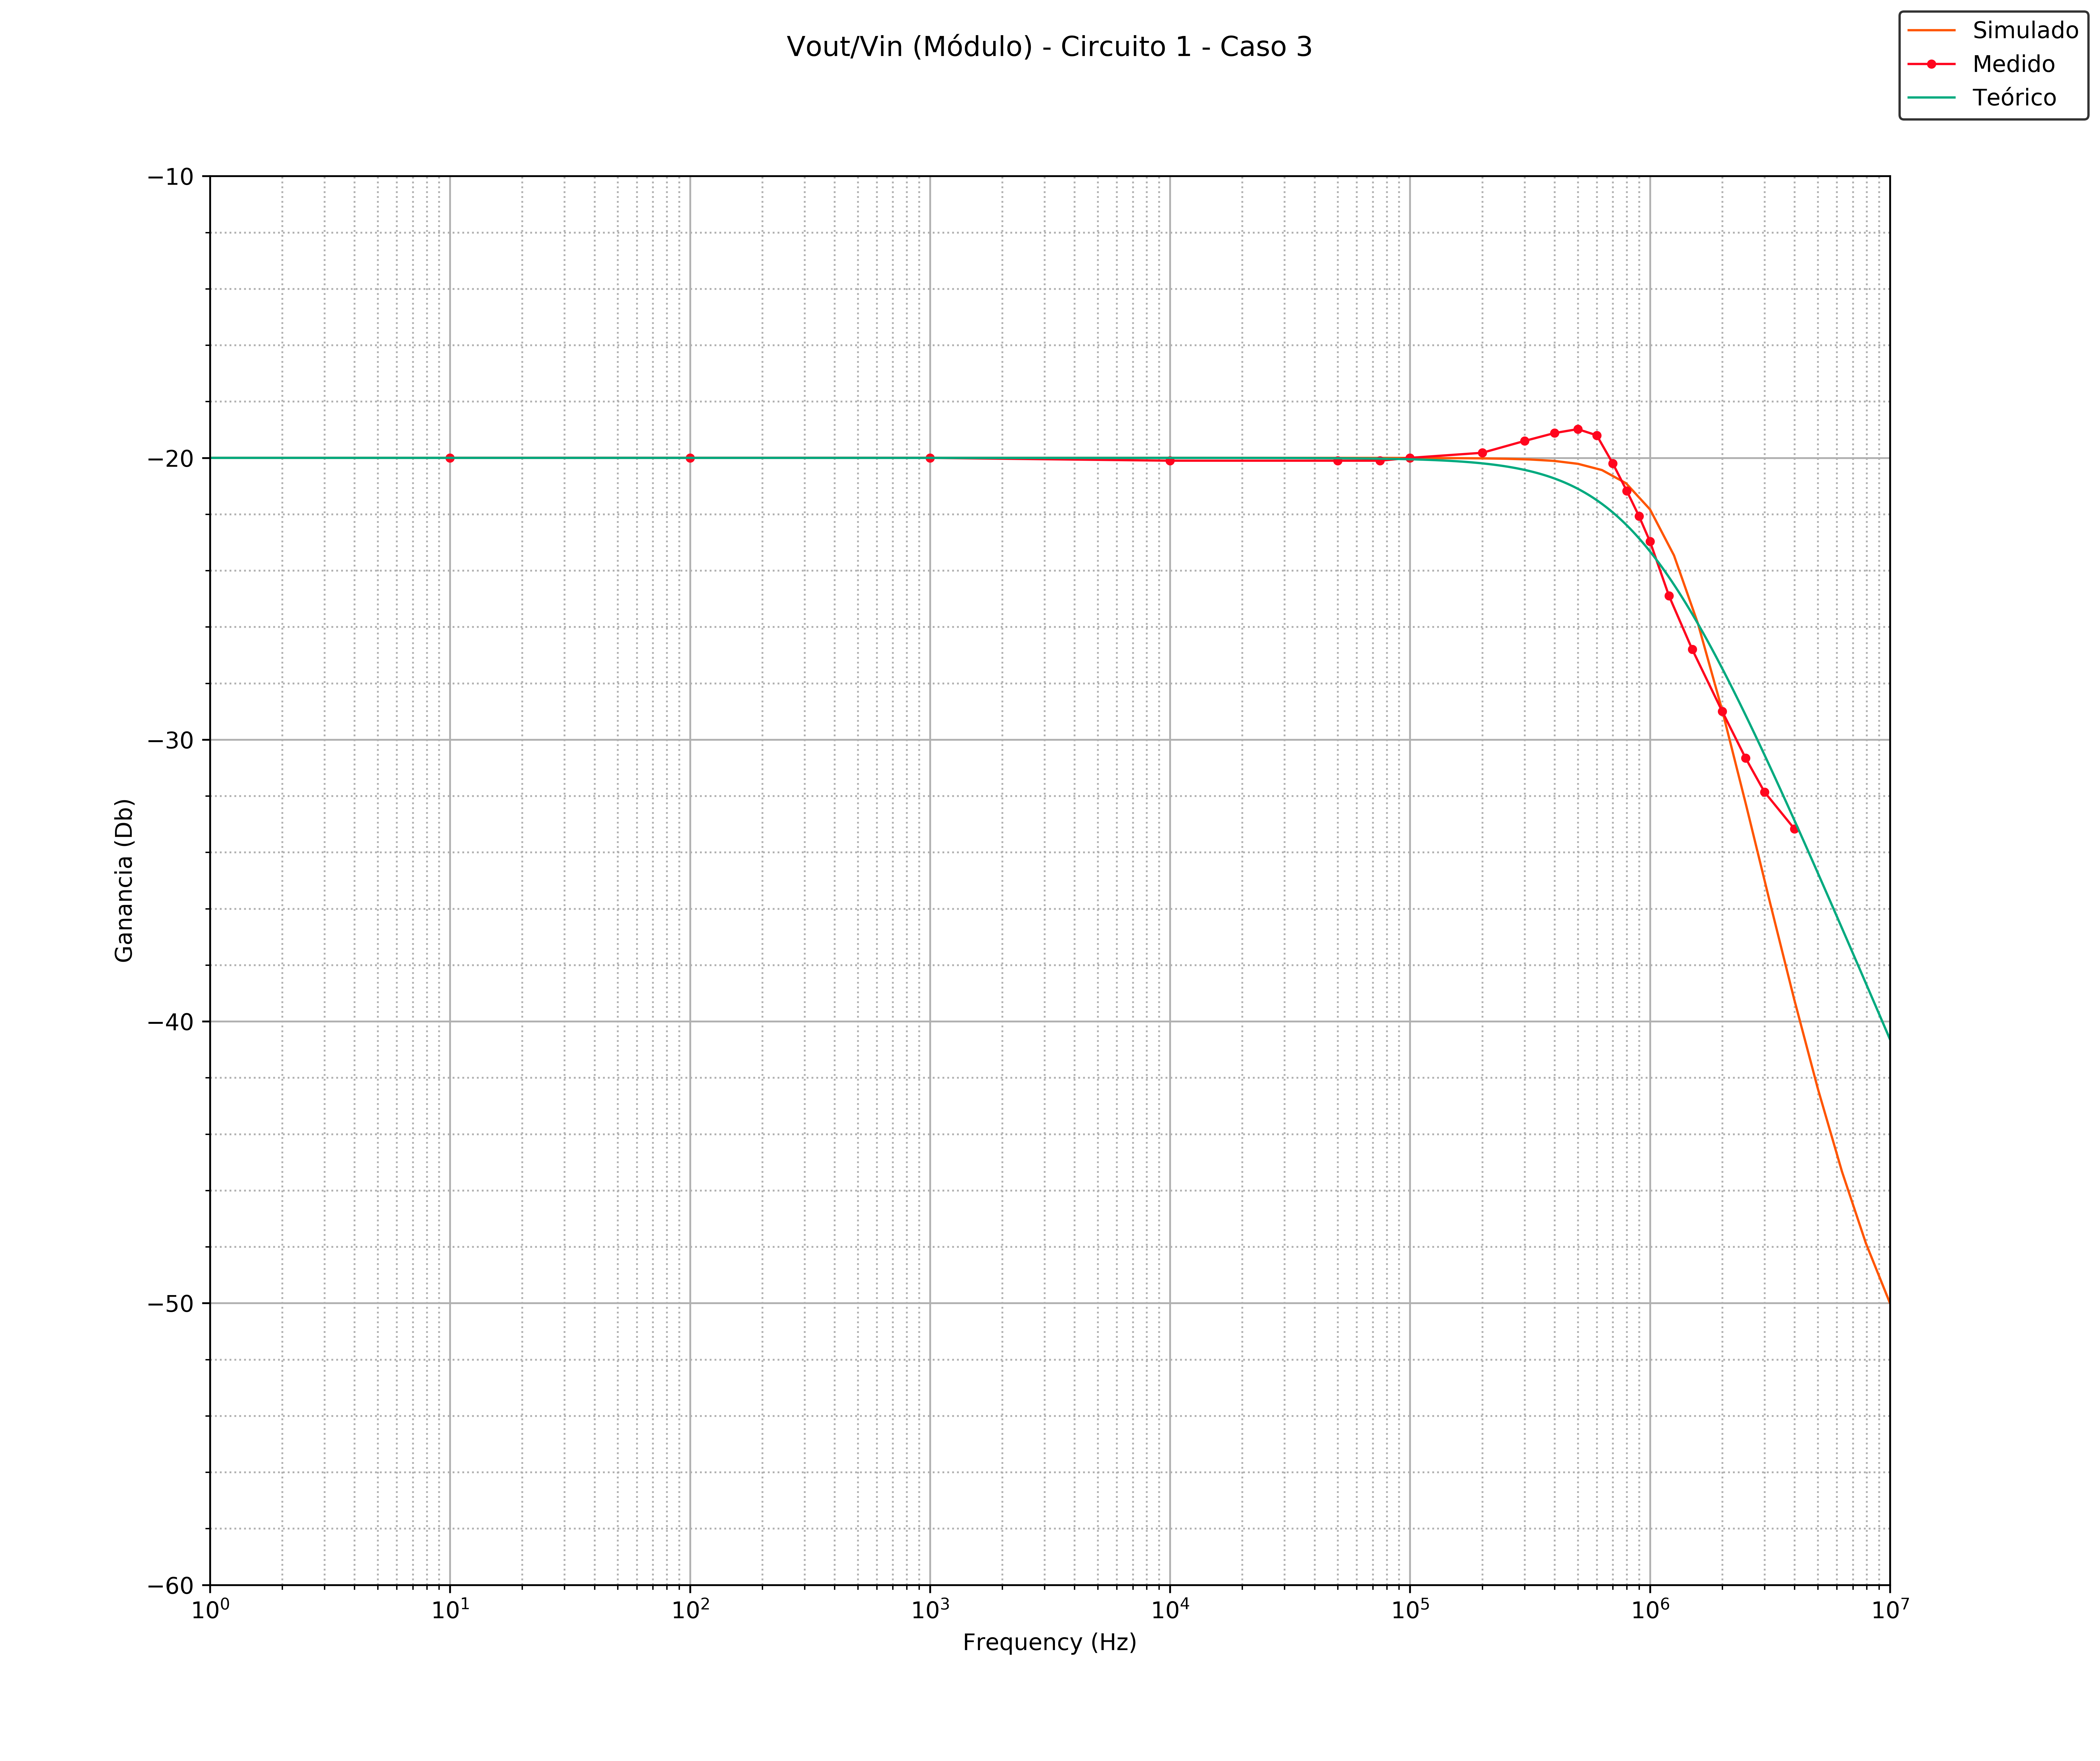
\includegraphics[width=10cm,height=10cm,keepaspectratio]{../EJ1/00GRAFICOS/c1c3/c1c3voviMod.png}
	\caption{Configuración inversora - Caso 3 - M\'odulo de$V_{out}/V_{in}$}	
	\label{c1c3voviM}
\end{figure}

\begin{figure}[H] %!ht
	\centering
	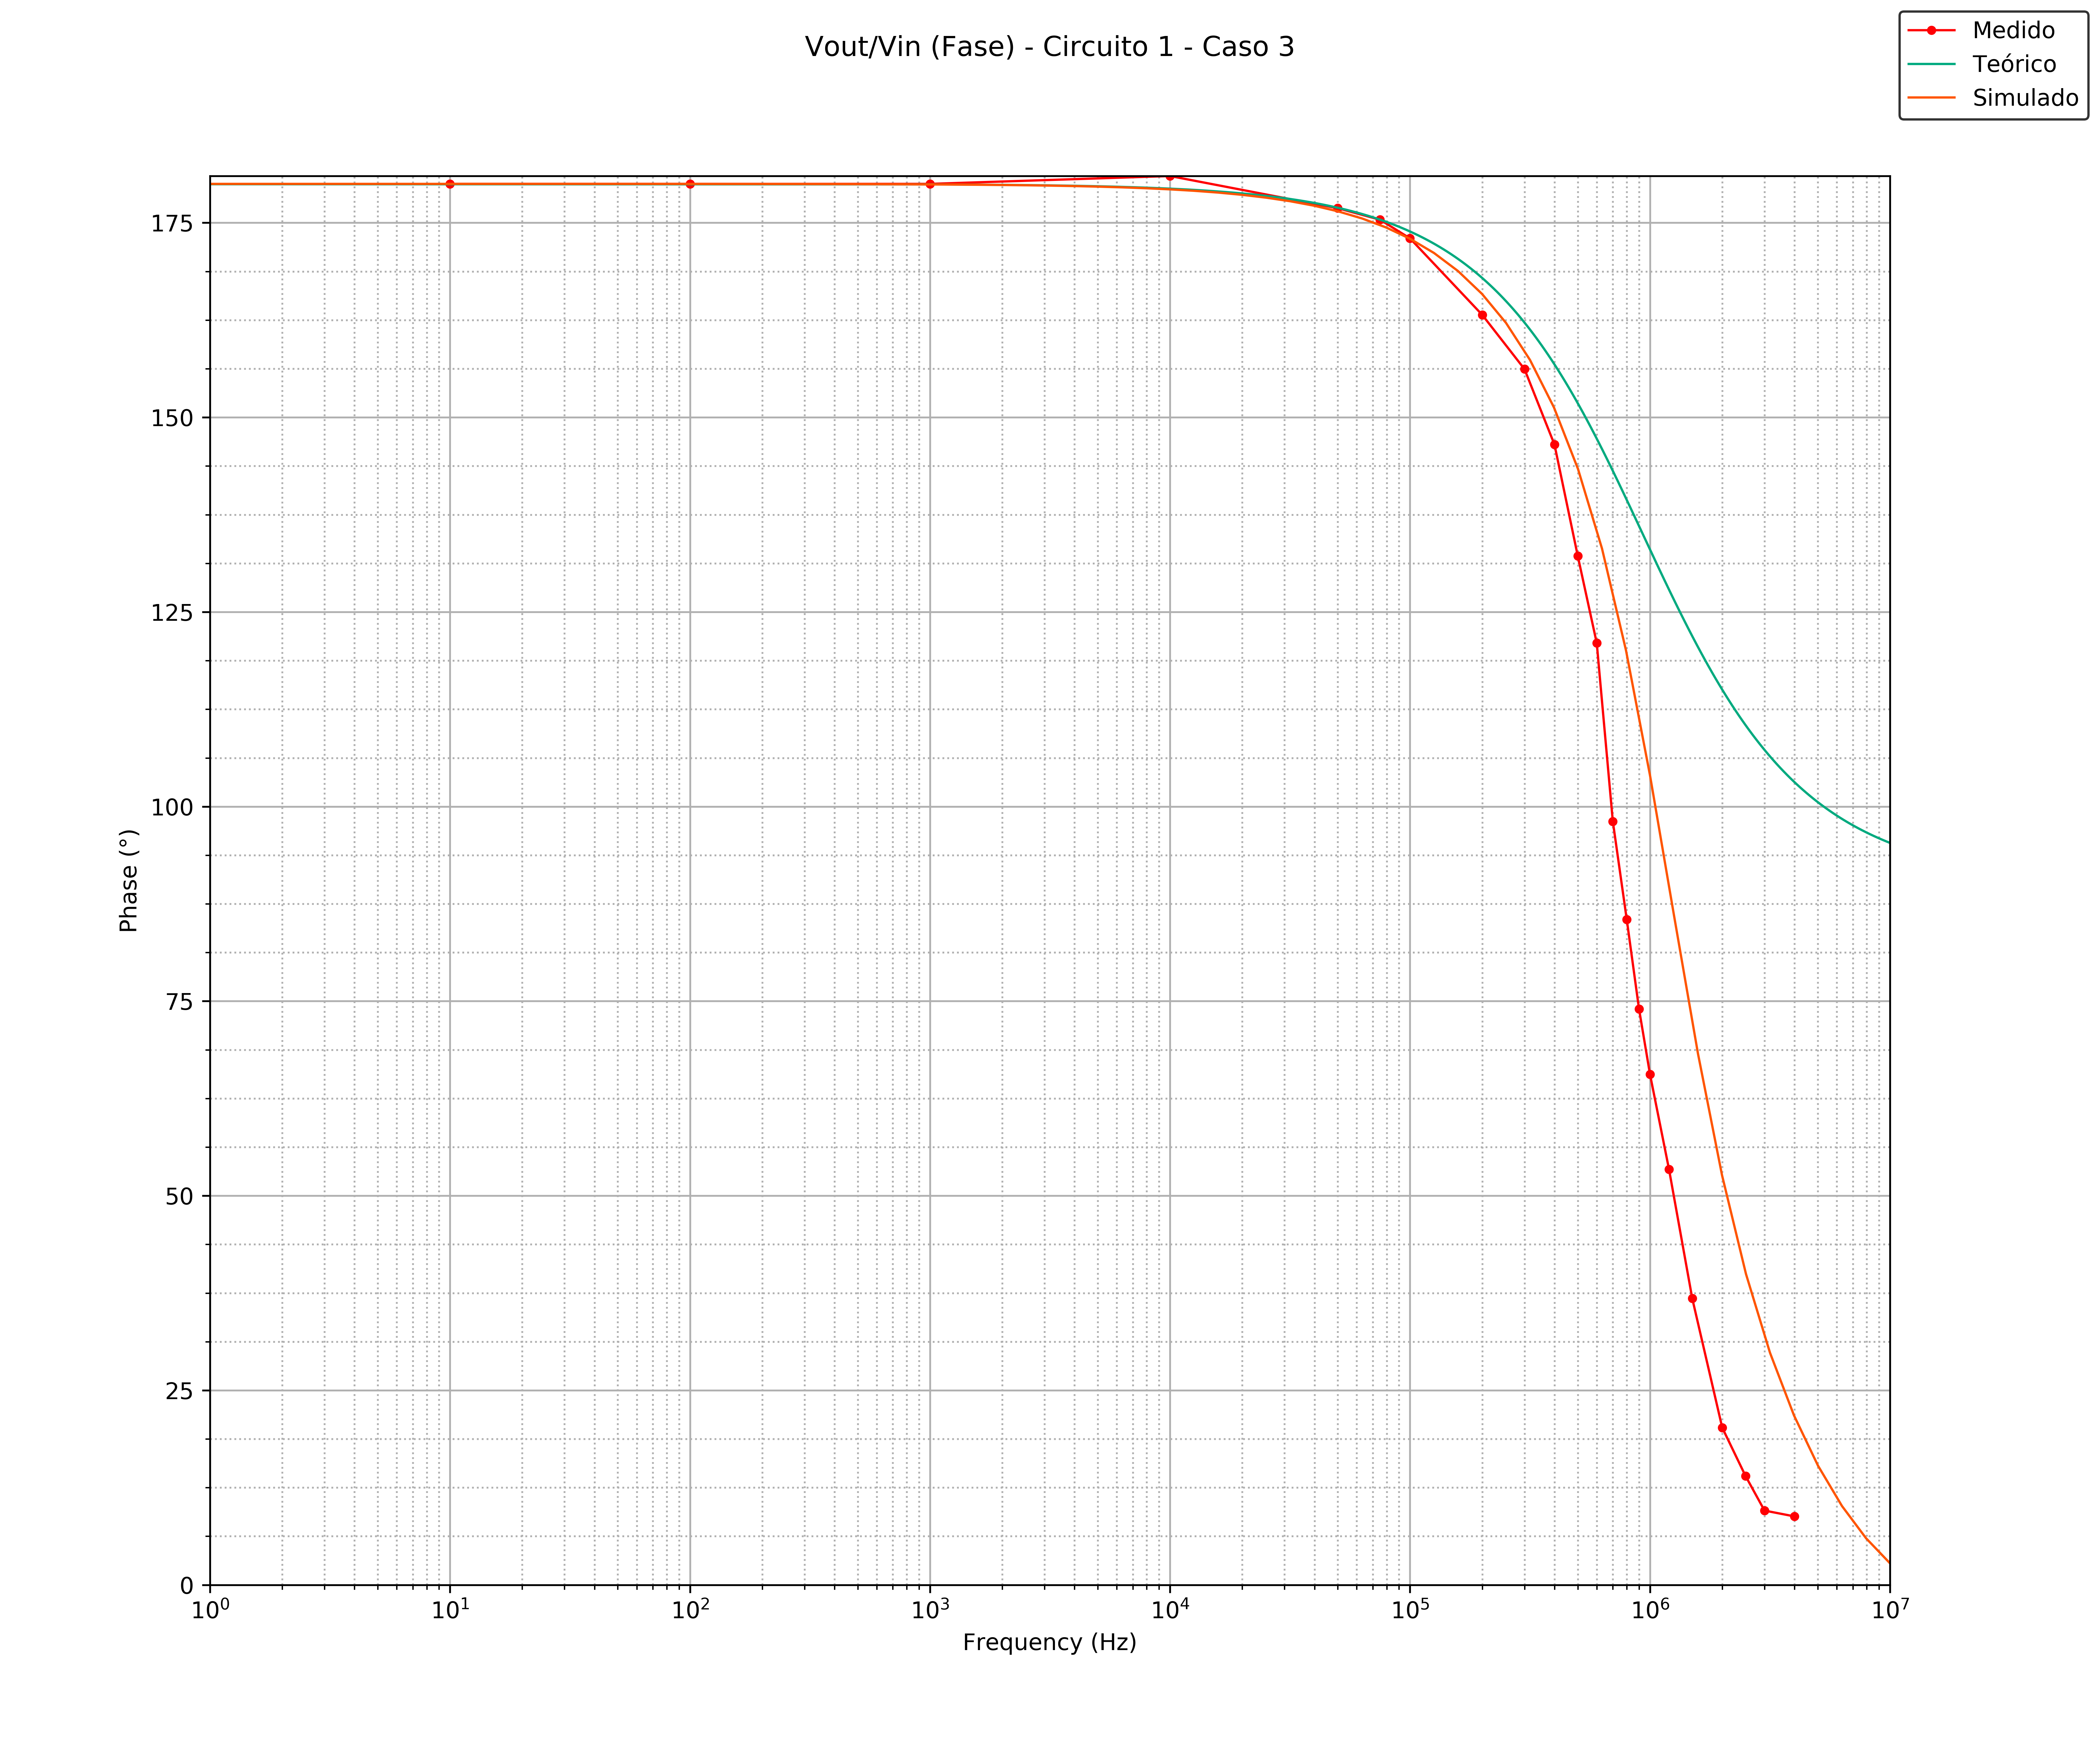
\includegraphics[width=10cm,height=10cm,keepaspectratio]{../EJ1/00GRAFICOS/c1c3/c1c3voviFASE.png}
	\caption{Configuración inversora - Fase de $V_{out}/V_{in}$}
	\label{c1c3voviP}
\end{figure}

\subsubsection*{Configuraci\'on no inversora}

\begin{figure}[H] %!ht
	\centering
	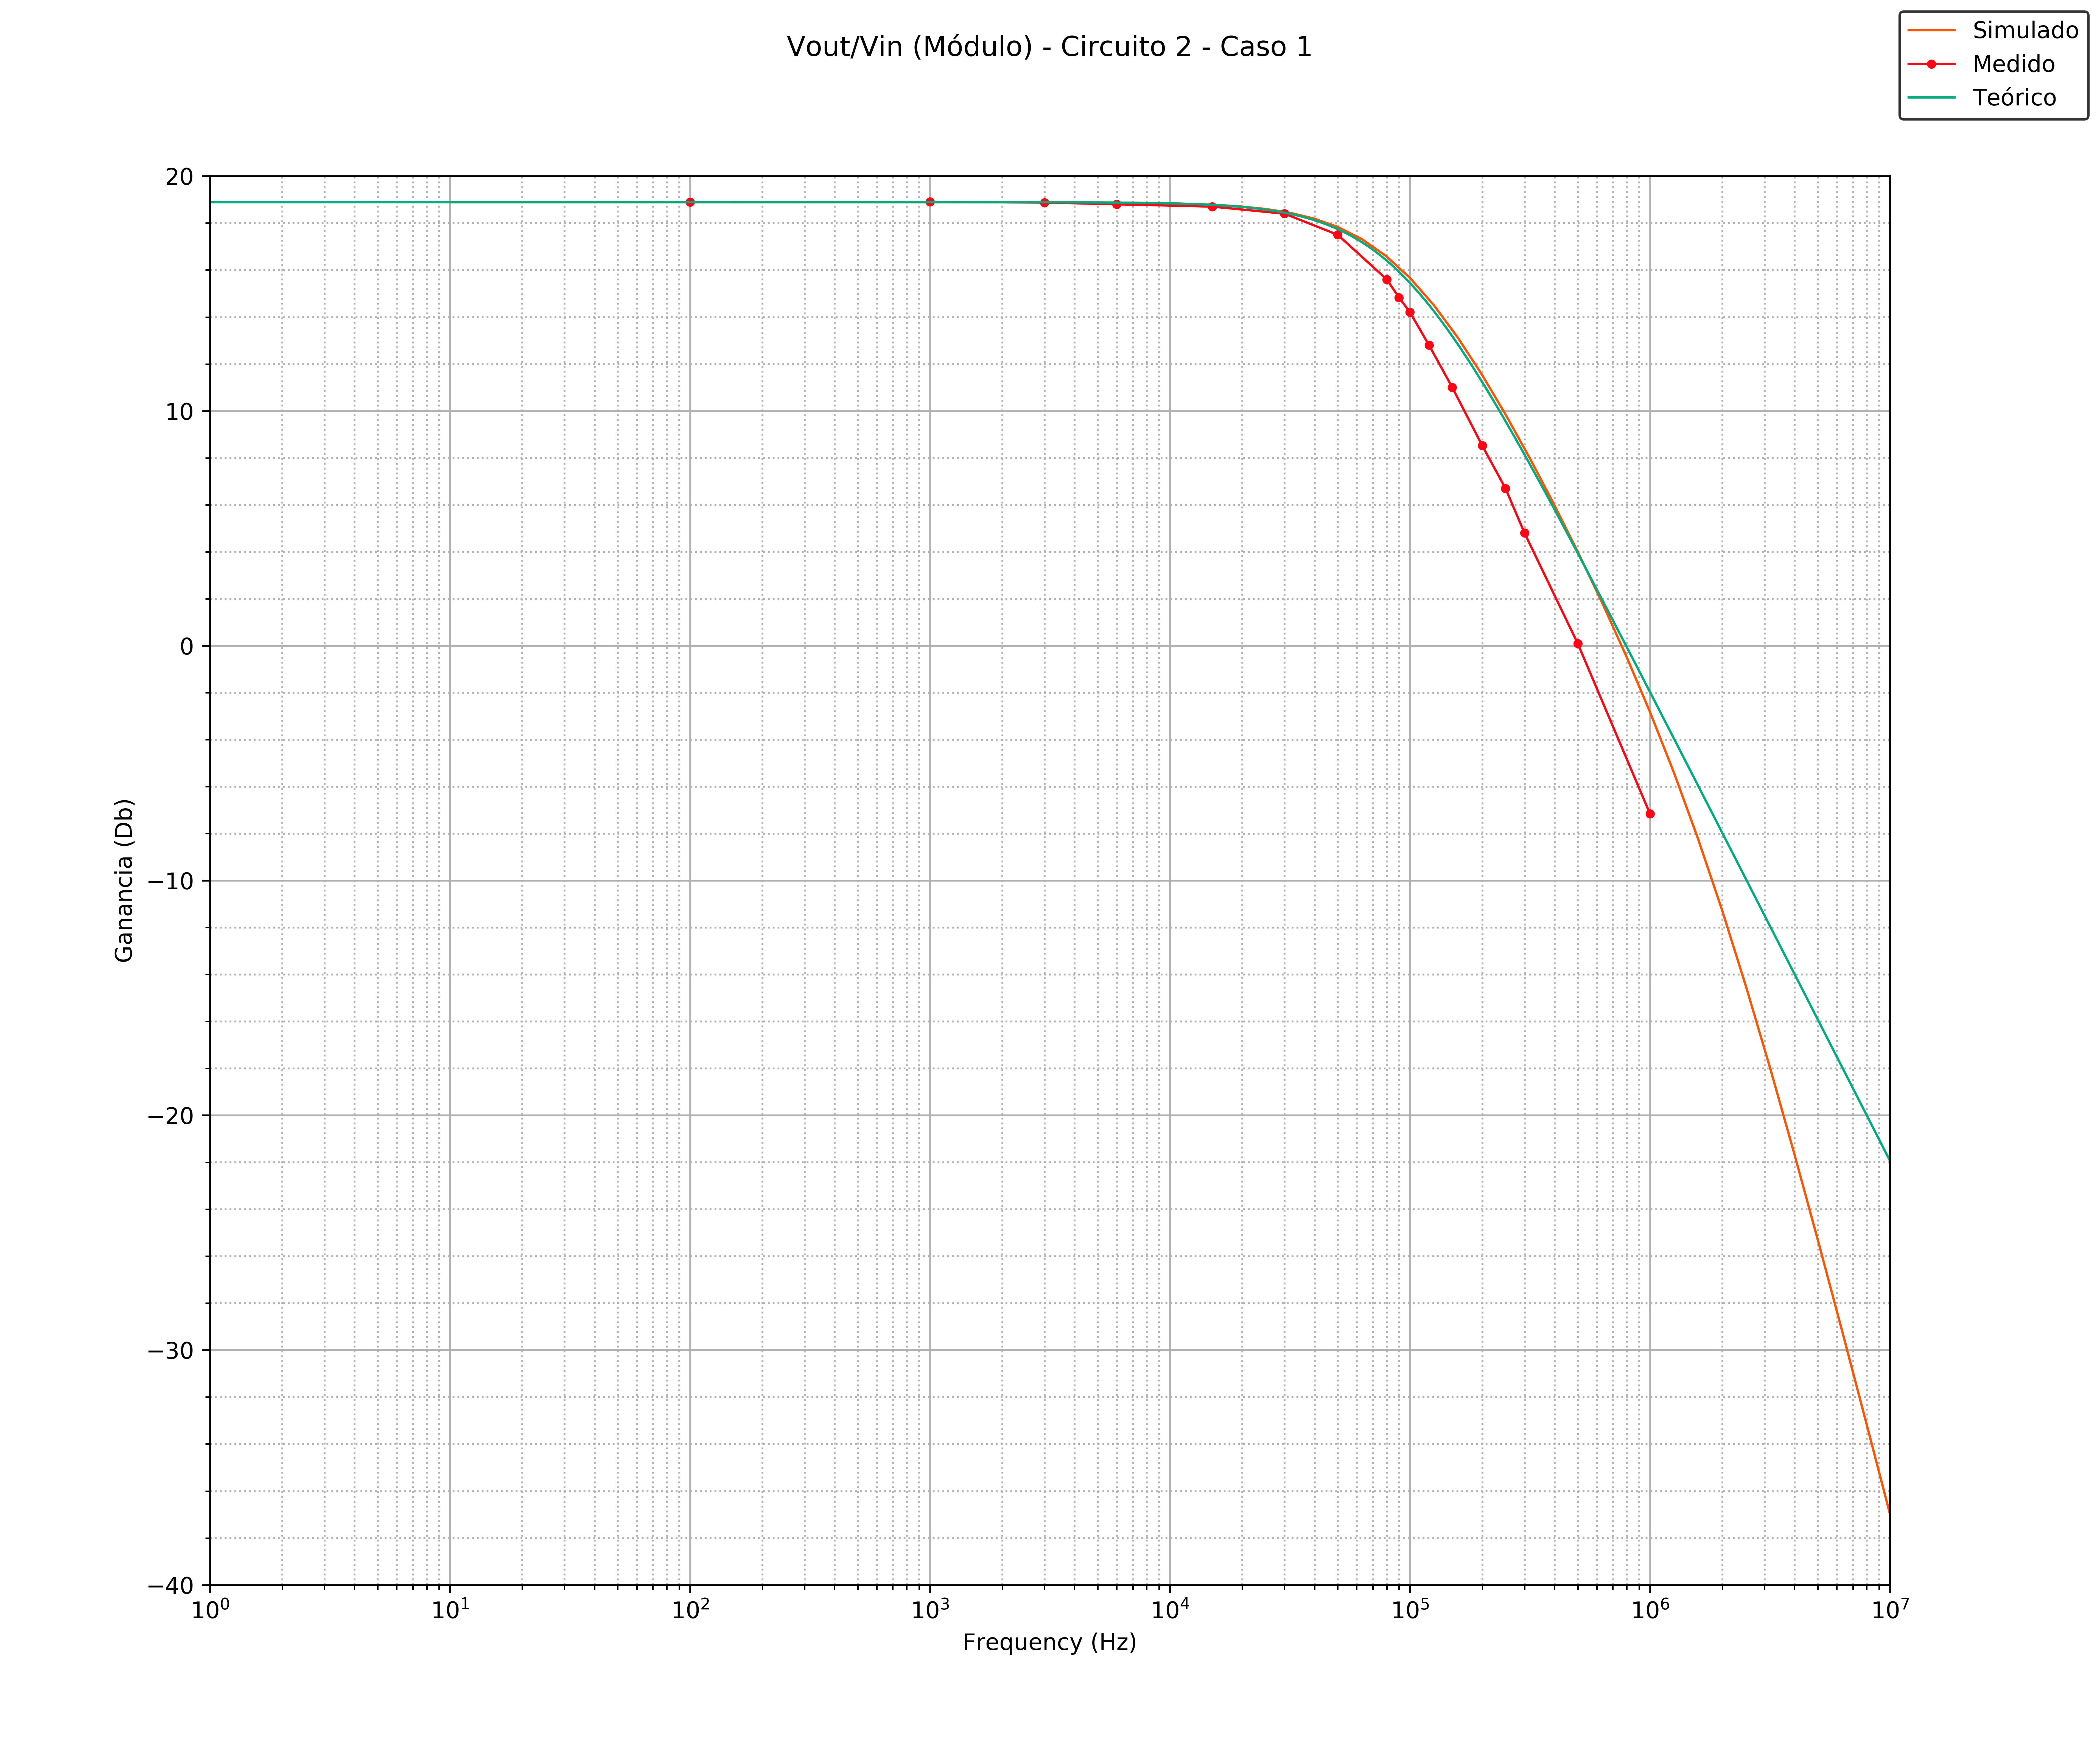
\includegraphics[width=10cm,height=10cm,keepaspectratio]{../EJ1/00GRAFICOS/c2c1/c2c1voviMod.png}
	\caption{Configuración no inversora - Caso 1 -  M\'odulo de $V_{out}/V_{in}$}
	\label{c2c1voviM}
\end{figure}

\begin{figure}[H] %!ht
	\centering
	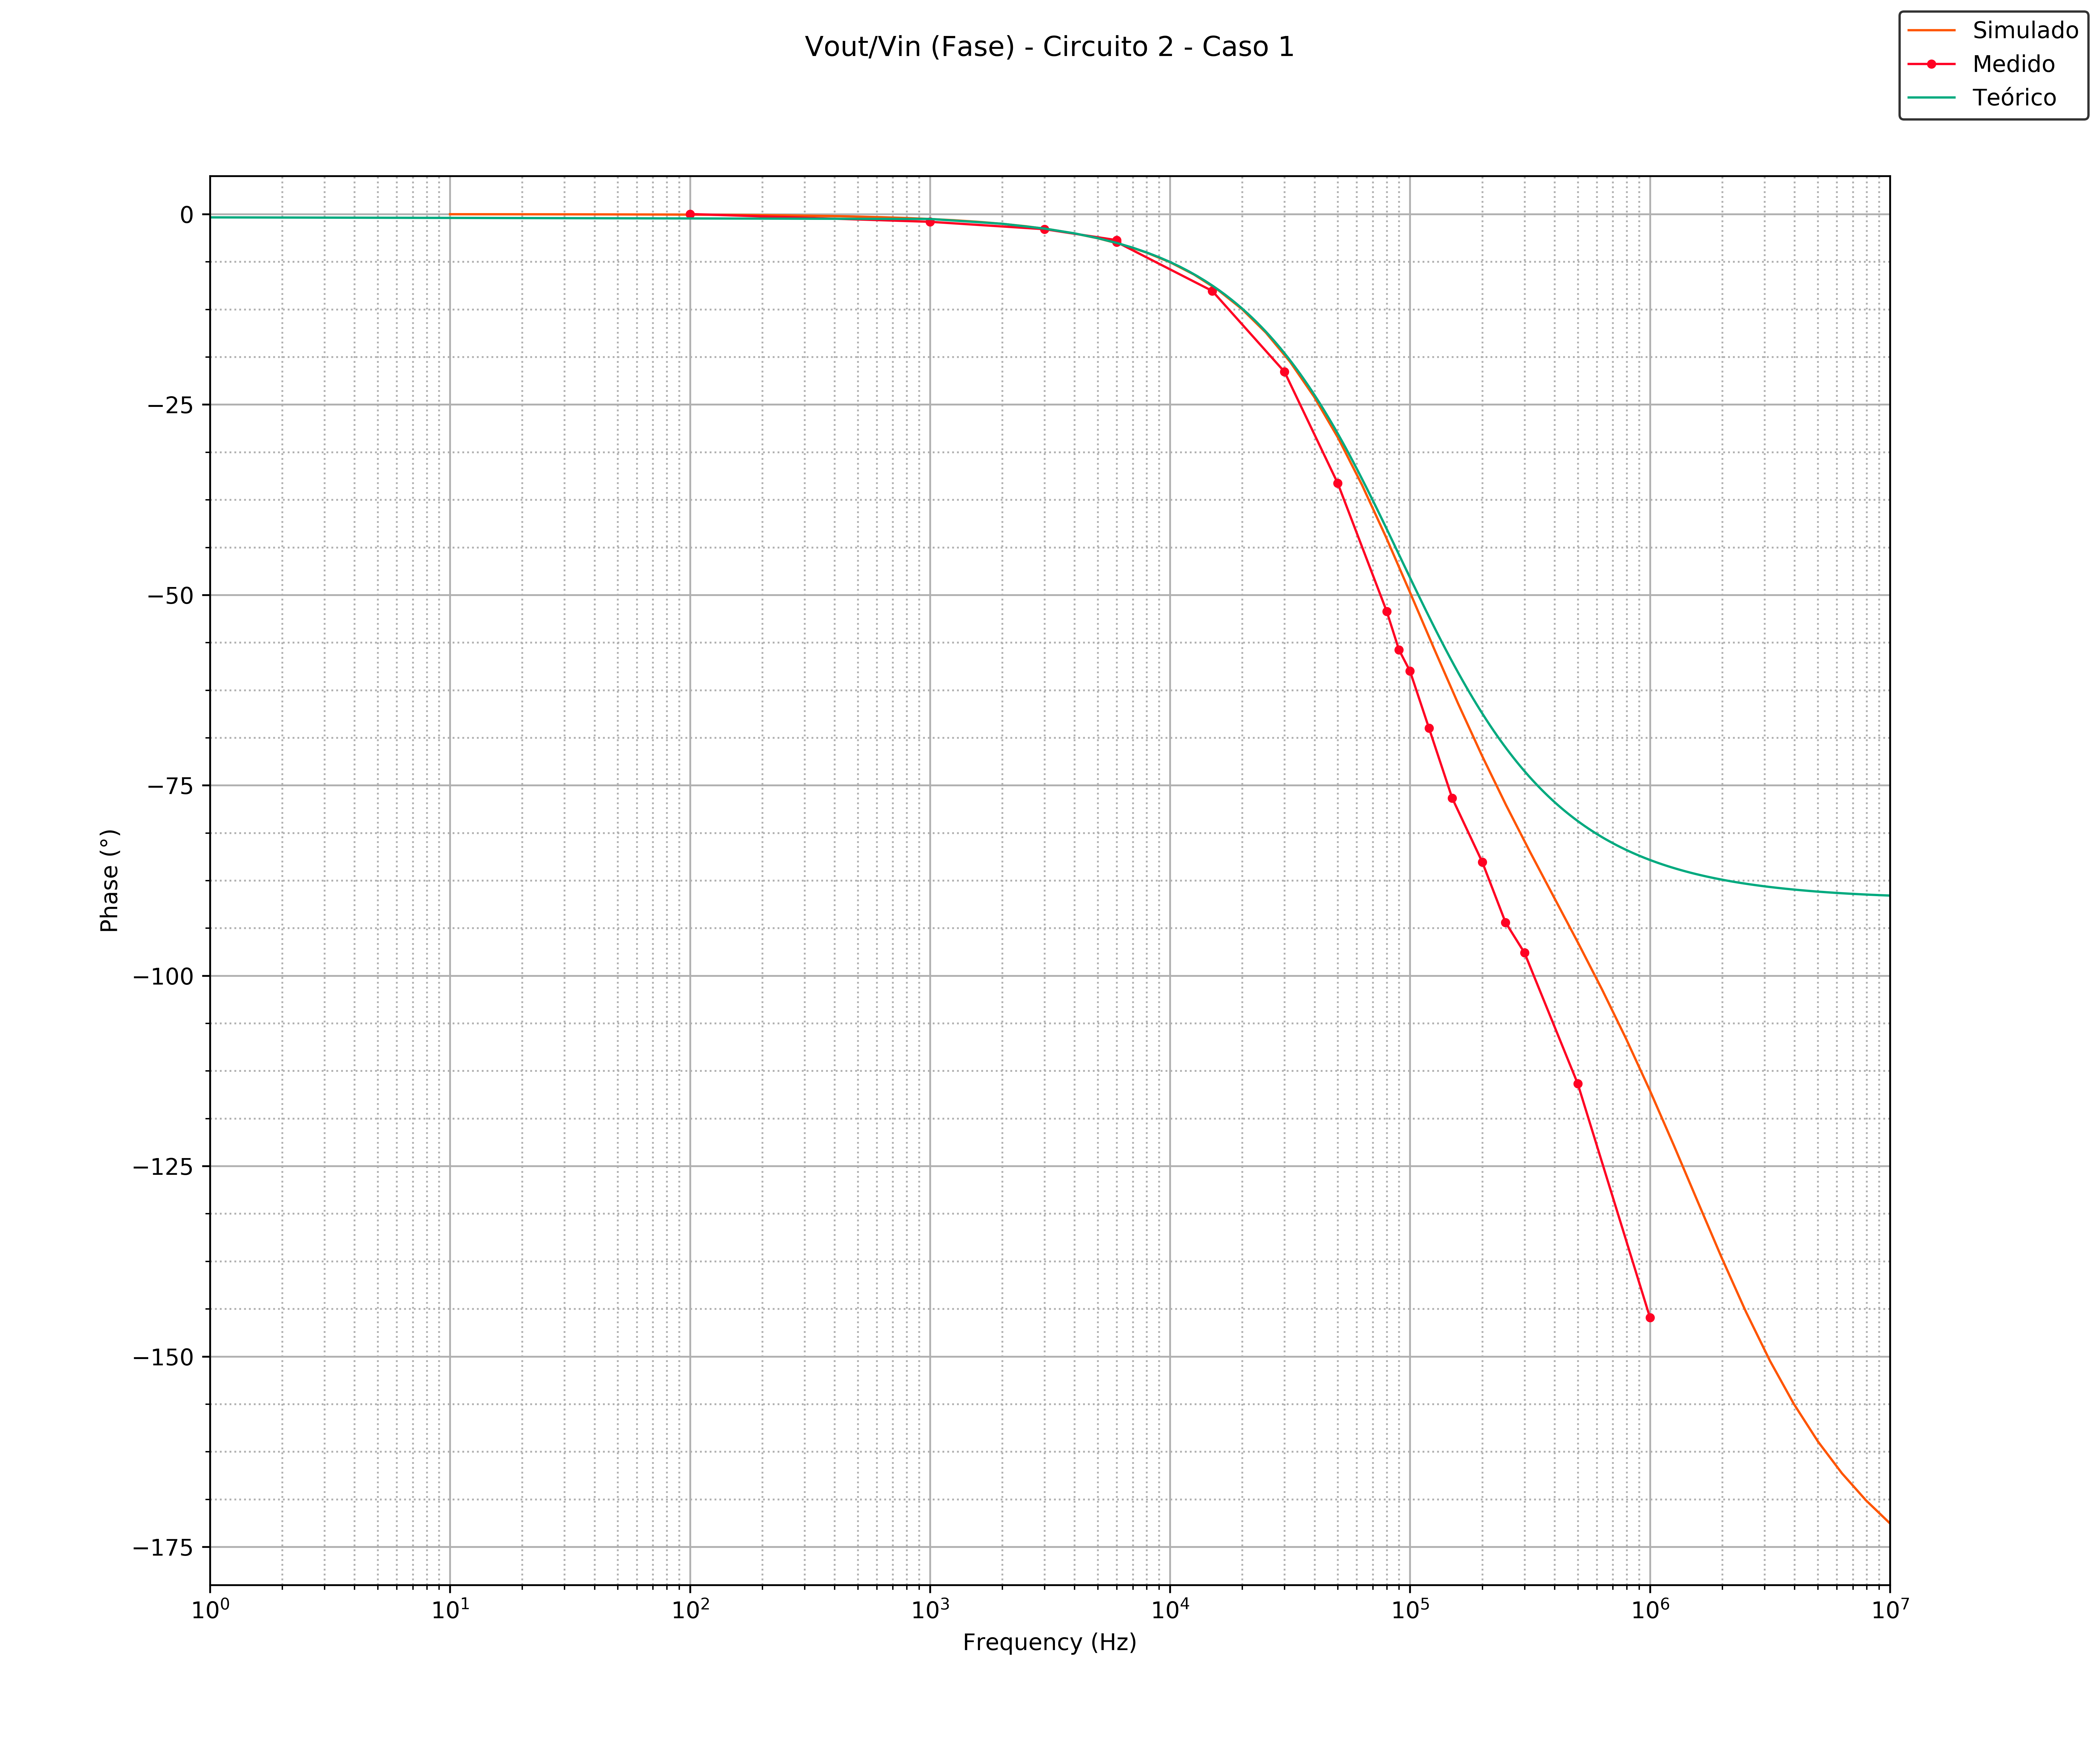
\includegraphics[width=10cm,height=10cm,keepaspectratio]{../EJ1/00GRAFICOS/c2c1/c2c1voviFASE.png}
	\caption{Configuración no inversora - Caso 1 - Fase de $V_{out}/V_{in}$}
	\label{c2c1voviP}
\end{figure}

\begin{figure}[H] %!ht
	\centering
	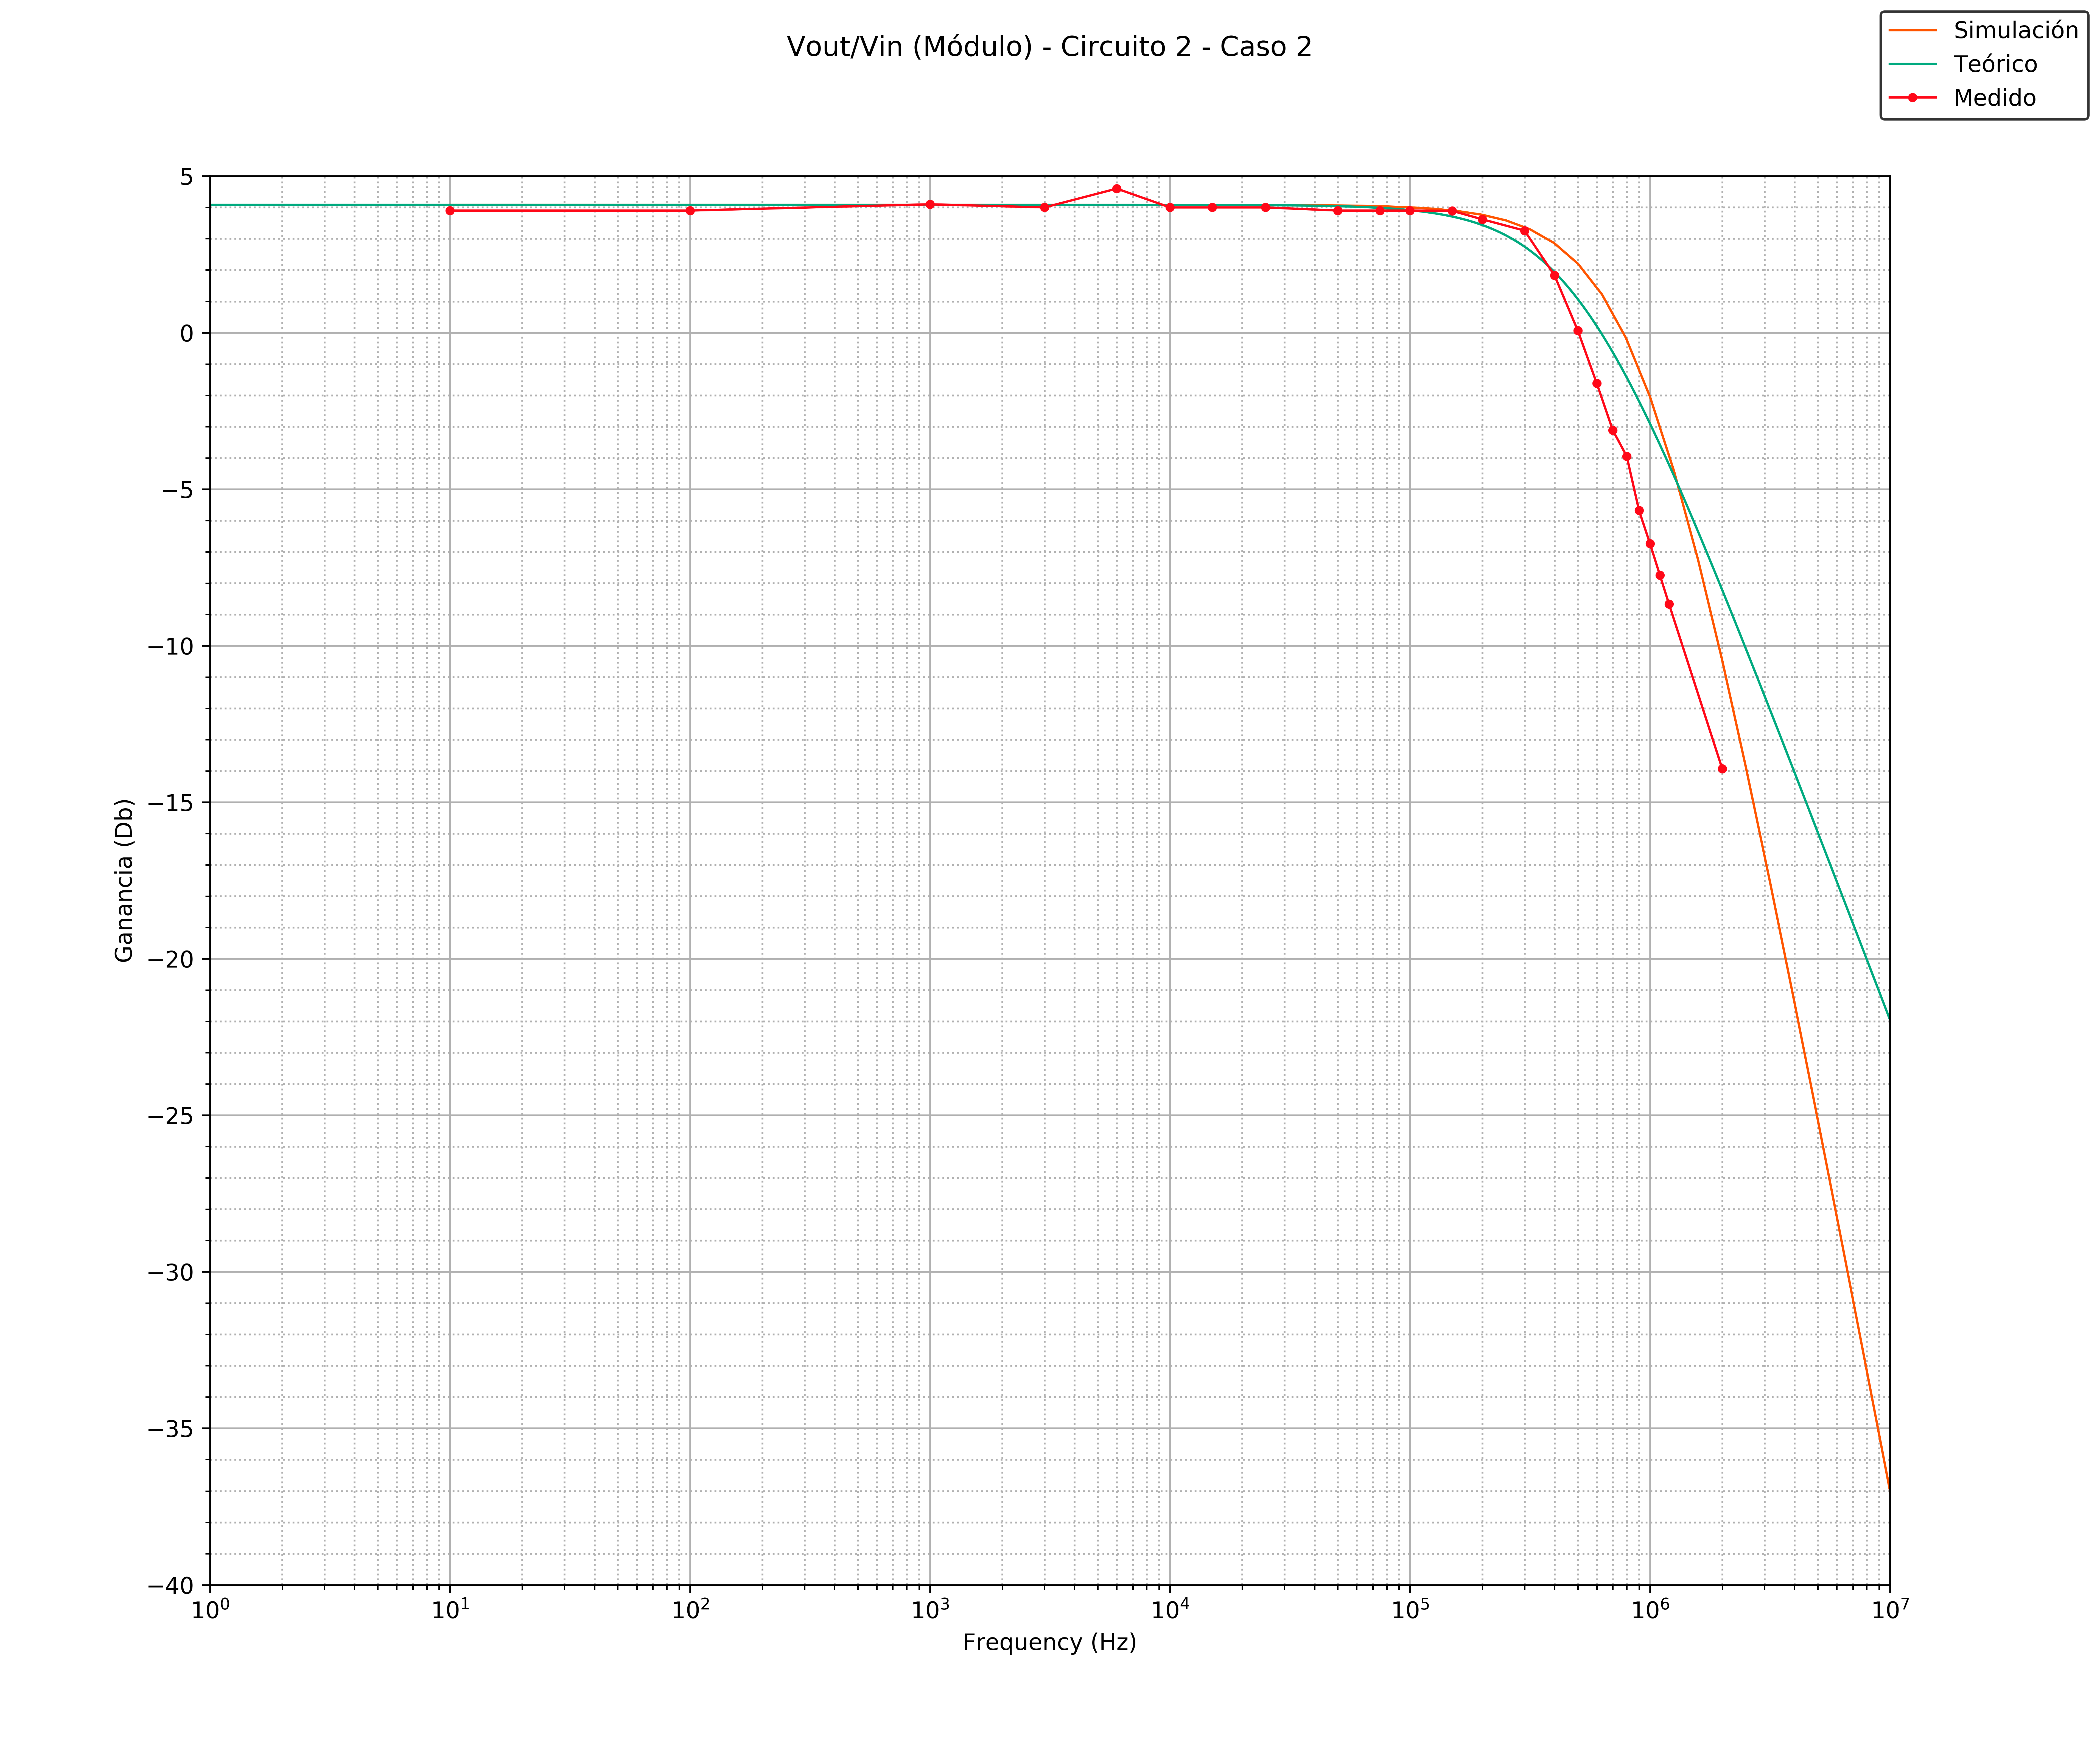
\includegraphics[width=10cm,height=10cm,keepaspectratio]{../EJ1/00GRAFICOS/c2c2/c2c2voviMod.png}
	\caption{Configuración no inversora - Caso 2 - M\'odulo de $V_{out}/V_{in}$}
	\label{c2c2voviM}
\end{figure}

\begin{figure}[H] %!ht
	\centering
	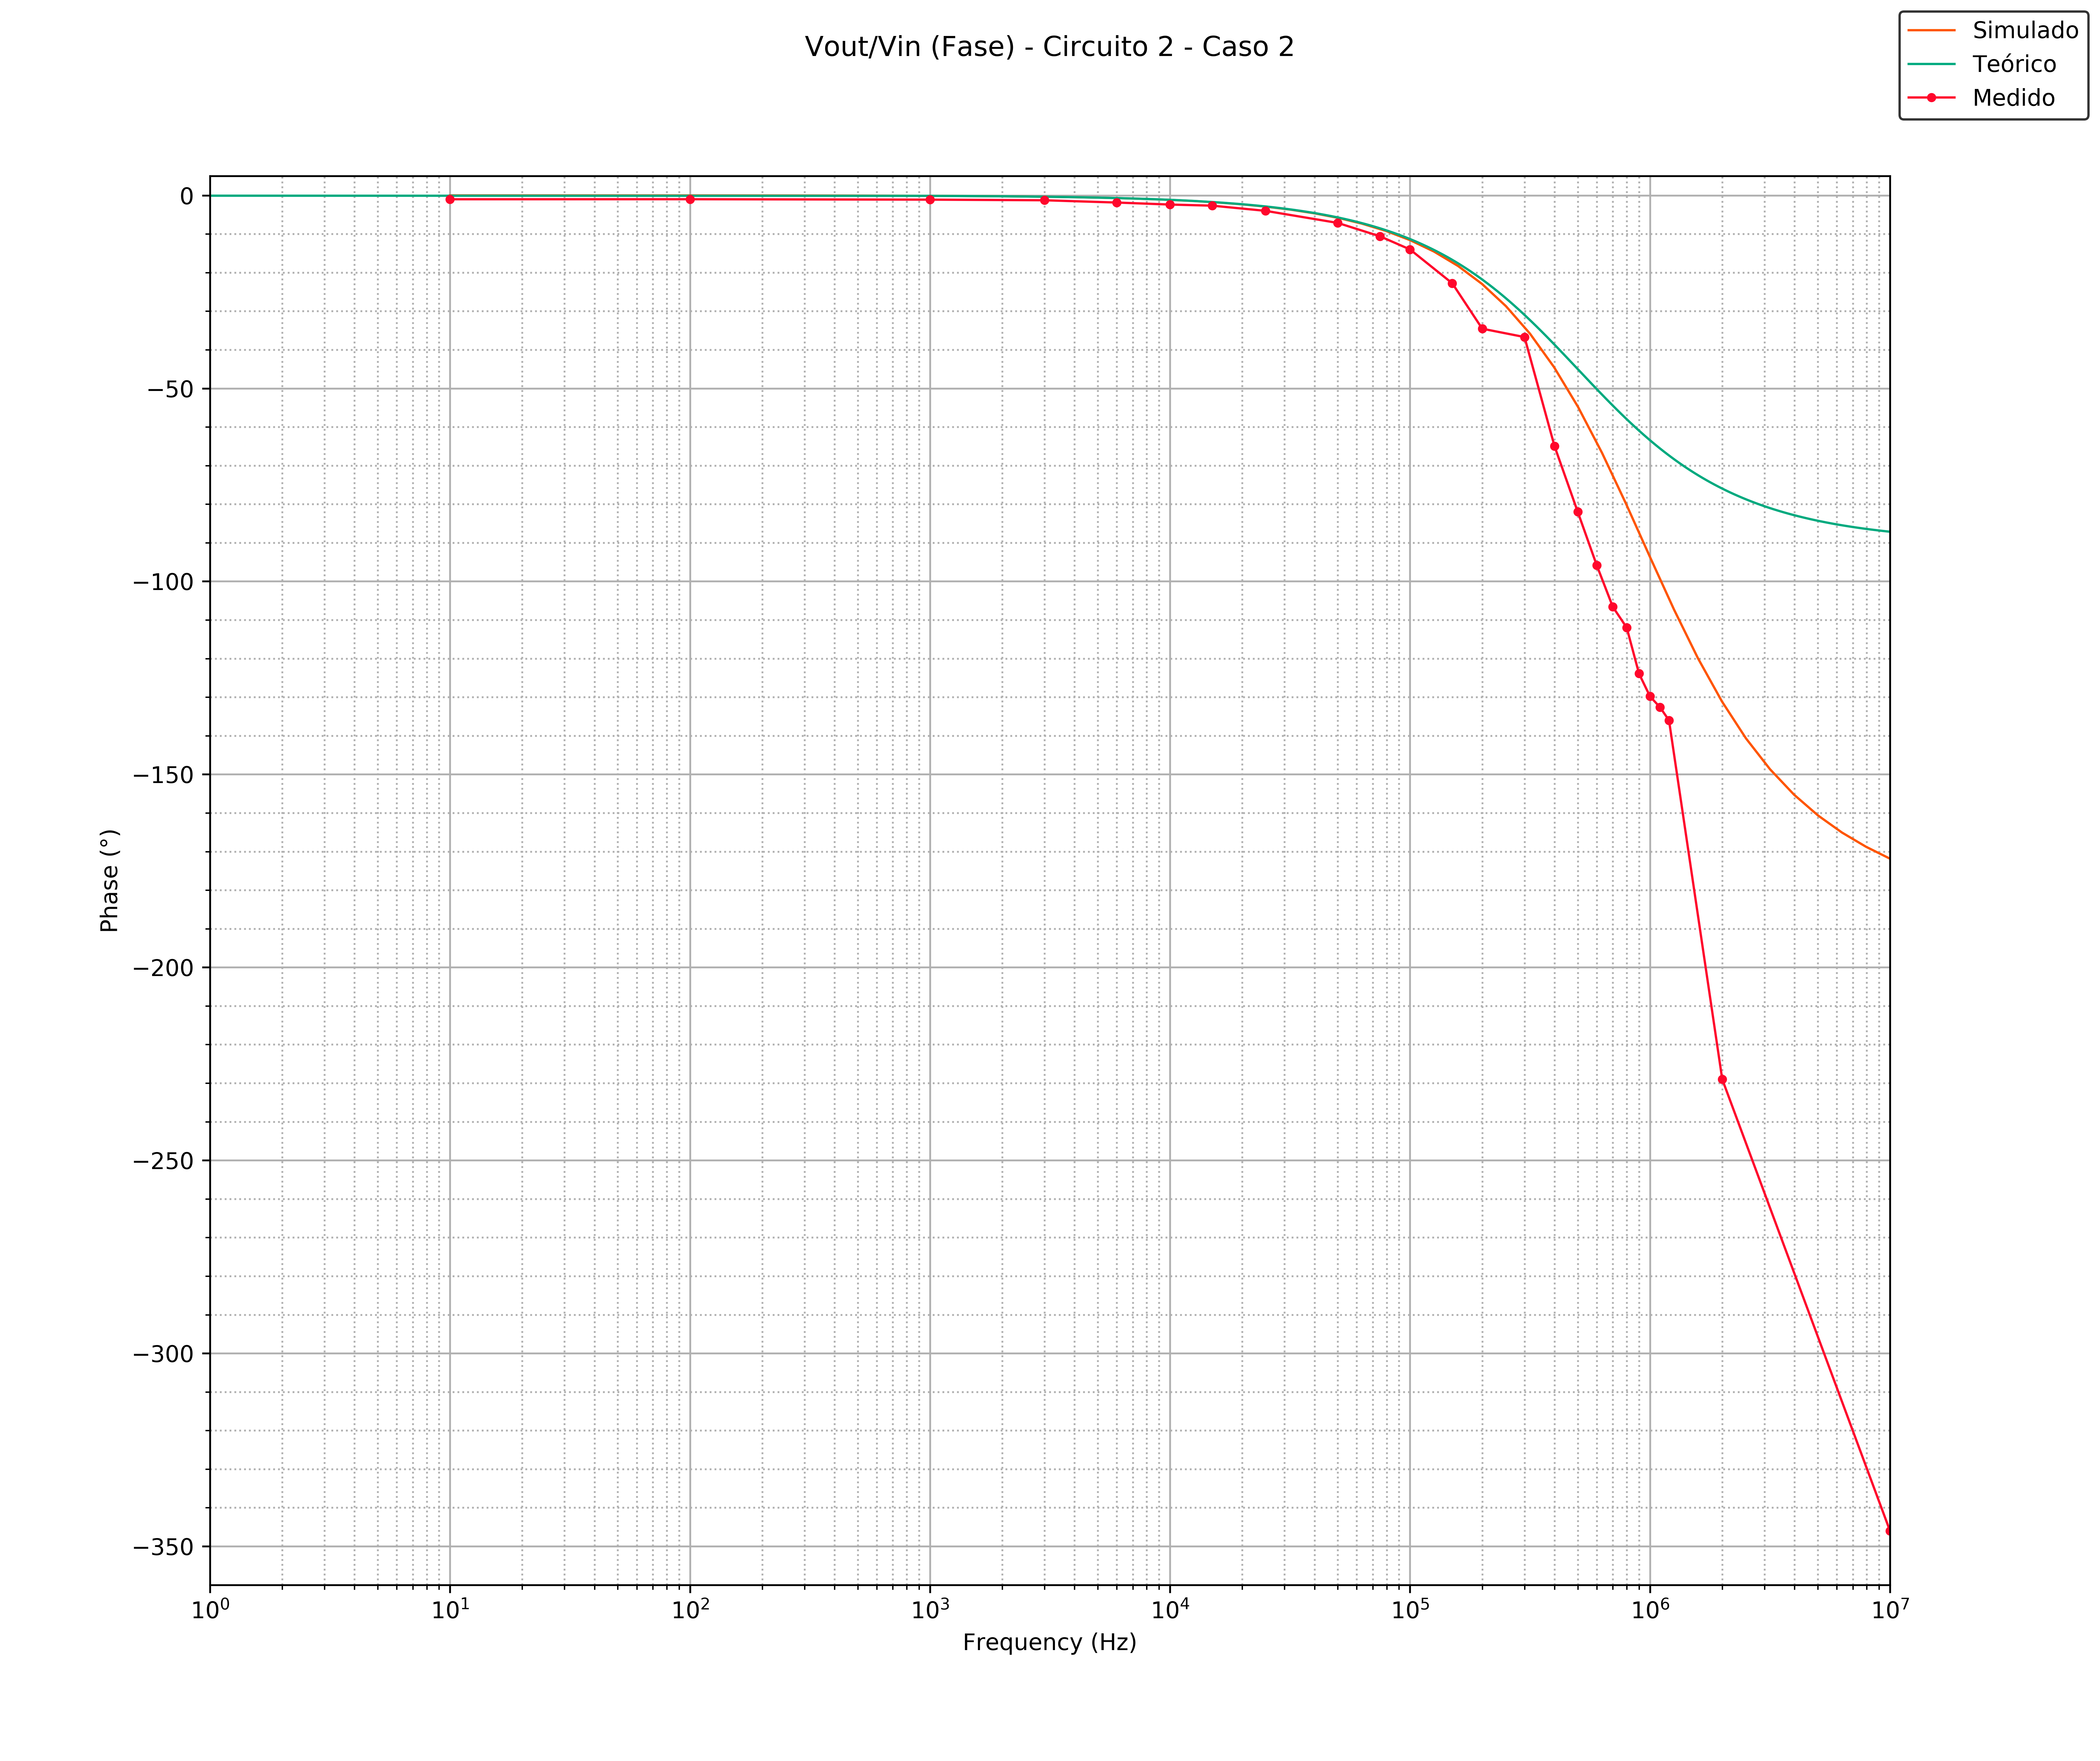
\includegraphics[width=10cm,height=10cm,keepaspectratio]{../EJ1/00GRAFICOS/c2c2/c2c2voviFASE.png}
	\caption{Configuración no inversora - Caso 2 - Fase de $V_{out}/V_{in}$}
	\label{c2c2voviP}
\end{figure}

%\begin{figure}[H] %!ht
%	\centering
%	\includegraphics[width=10cm,height=10cm,keepaspectratio]{../EJ1/00GRAFICOS/c2c3/c2c3voviMod.png}
%	\caption{Configuración no inversora - Caso 3 - M\'odulo de $V_{out}/V_{in}$}	
%	\label{c2c3voviM}
%\end{figure}

\begin{figure}[H] %!ht
	\centering
	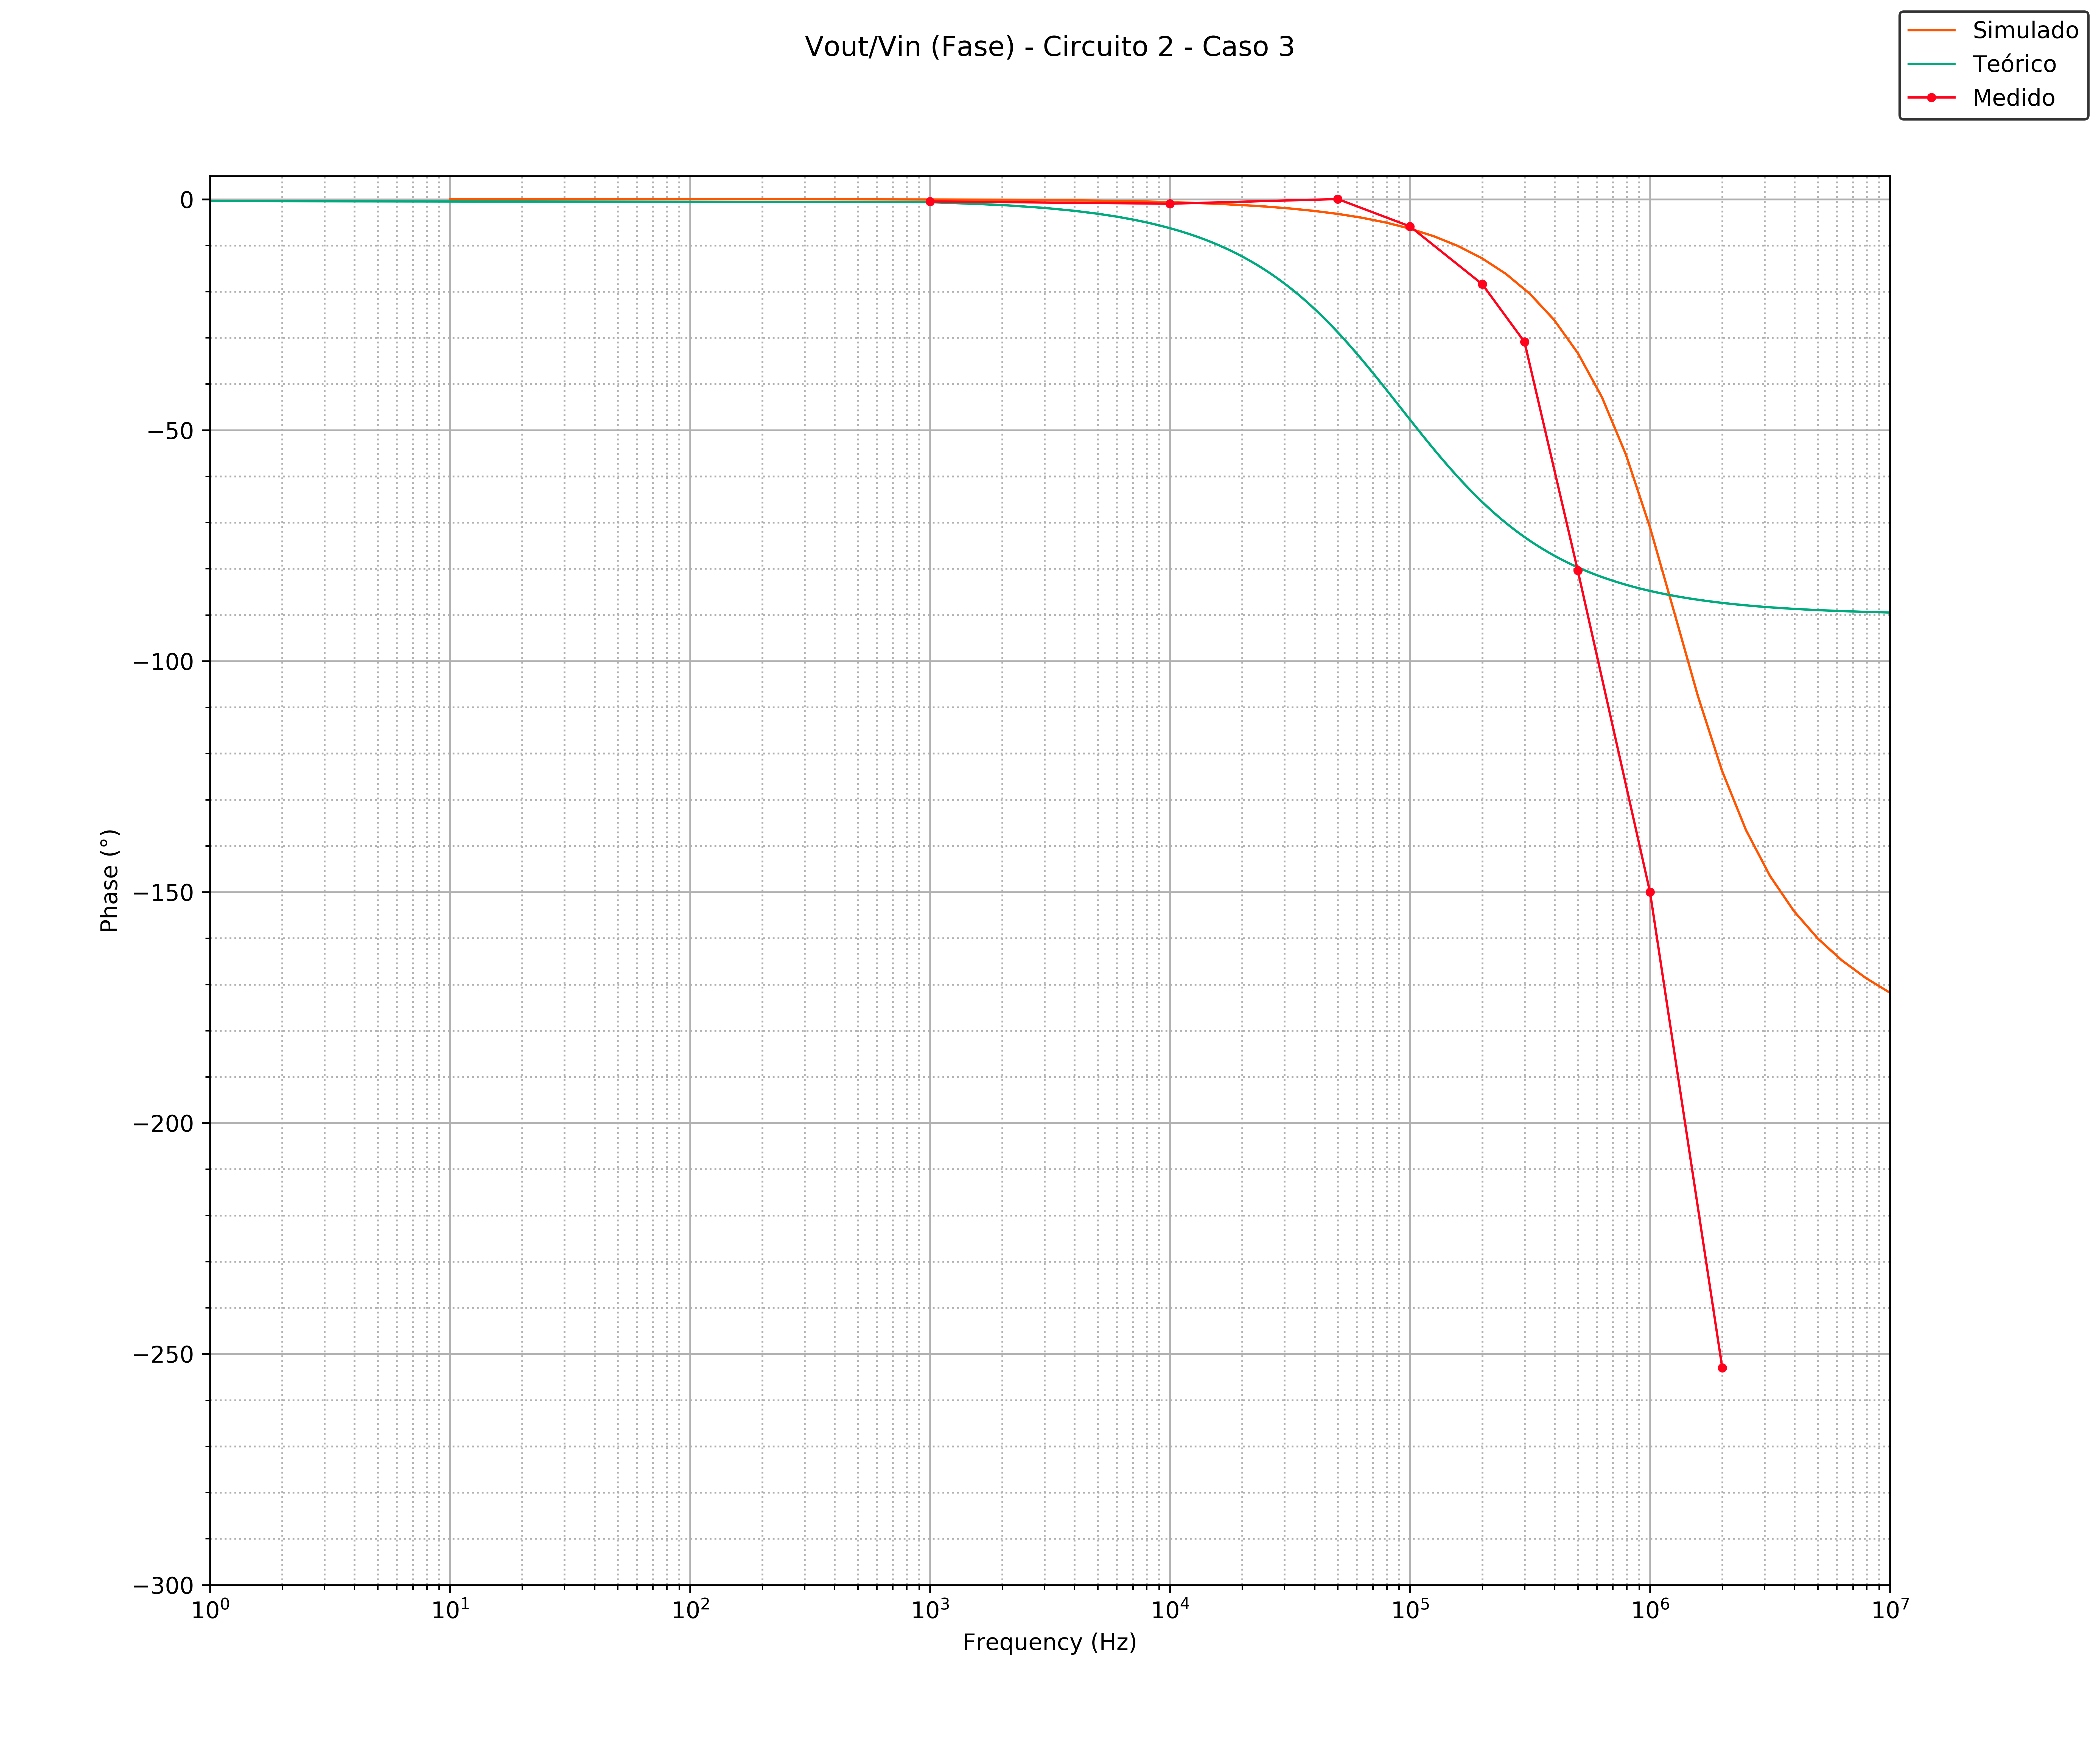
\includegraphics[width=10cm,height=10cm,keepaspectratio]{../EJ1/00GRAFICOS/c2c3/c2c3voviFASE.png}
	\caption{Configuración no inversora - Caso 3 - Fase de $V_{out}/V_{in}$}
	\label{c2c3voviP}
\end{figure}



